\documentclass[titlepage,openright,letterpaper,12pt]{book}
\usepackage{config/entete}
\usepackage{config/commandes} % Load les packages et définit des commandes.
\usepackage{config/notation} % Load les packages et définit des commandes.

%=============================================================================%

% On crée des bools qui sont False par défaut.
\newtoggle{VersionLivre}
\newtoggle{LivrePGChVide}
\newtoggle{ForceEntete}
\newtoggle{AuteureFemme}
\newtoggle{MemoirePasThese}
\newtoggle{useCustomFonts}
\newtoggle{generatePDFa}
\newtoggle{IntroConcluSansNombre}

% Switchboard, l'endroit ou on ajuste les toggles.
% Décommenté -> True; commenté -> False

%\toggletrue{VersionLivre}          % Décommenter pour faire la version livre
%\toggletrue{LivrePGChVide}         % Page gauche de chapiter vide en mode livre.
%\toggletrue{ForceEntete}            % Entête même pour version électronique.
%\toggletrue{AuteureFemme}          % Décommenter si l'auteur est une femme.
%\toggletrue{MemoirePasThese}       % Décommenter dans le cas d'un mémoire.
\toggletrue{IntroConcluSansNombre}  % Intro et conclusion non numérotées
\toggletrue{useCustomFonts}         % Fonts différents, voir switchboard.tex.
%\toggletrue{generatePDFa}           % Génère un PDFa plutôt qu'un PDF standard.

%=============================================================================%

\title{
  Une odyssée de la communication classique à la tolérance aux fautes quantique
} % Pour la page de titre/jury.
\author{Maxime Tremblay}  % Idem
\Organisation{UNIVERSITÉ de SHERBROOKE}
\Location{Sherbrooke, Québec, Canada}
\ResumeCourt{}
\date{\today}       % Idem
\MotsClefs{Mots-Clefs \sep Pertinents \sep avec séparateurs}

% On cache le code exécuté dans ce fichier parce qu'il est laid et impertinent.
  \begin{comment}
\end{comment}

%=============================================================================%

\makeatletter   % Permet d'accèder aux variables @

%=============================================================================%

    % PDFA-1b/Hyperref
    \iftoggle{generatePDFa}
    {
        % PDF/A stuff (experimental)
        \usepackage[a-1b]{pdfx}
    }
    {
        \newcommand{\sep}{, }
    }%
        \begin{filecontents*}[overwrite]{\jobname.xmpdata}
\Title          {\@title}
\Author         {\@author}
\Subject        {\ResumeCourt}
\Org            {\Organisation}
\Keywords       {\MotsClefs}
\PublicationType{book}
        \end{filecontents*}%
        % Couleurs moins intenses, https://ethanschoonover.com/solarized/
        \definecolor{solblue}{HTML}{268bd2}
        \definecolor{solred}{HTML}{dc322f}
        \definecolor{solviolet}{HTML}{6c71c4}
        \definecolor{solmagenta}{HTML}{d33682}
        \definecolor{solcyan}{HTML}{2aa198}
        \definecolor{solorange}{HTML}{cb4b16}
        \definecolor{solyellow}{HTML}{b58900}
        \definecolor{solgreen}{HTML}{859900}
        % Hyperrefs
        \usepackage{hyperref}
        \hypersetup{
            pdfauthor={\@author},
            pdftitle={\@title},
            pdfsubject={\ResumeCourt},
            pdfkeywords={\MotsClefs},
            % pdfa,
            colorlinks=true,
            breaklinks=true,
            urlcolor=solmagenta,
            linkcolor=solblue,
            citecolor=solcyan,
            bookmarksopen=true,
            unicode=true
        }
        \usepackage[hyperpageref]{backref}      % Backrefs!
        \renewcommand{\backref}[1]{[cf.~p.~#1]} % Volé cette ligne à Samuel Boutin
        \usepackage{bookmark}
        \usepackage{cmap} % Doit être après hyperref pour être compatible avec pdf-a

%=============================================================================%

    \iftoggle{useCustomFonts}
    {   
        % Deux prochaines lignes -> Pagella et Mathpazo
        %\usepackage{mathpazo} % utilise Palatino pour les mathématiques (mettre en premier)
        %\usepackage{tgpagella} % utilise la police TeX Gyre Pagella

        % Deux prochaines lignes -> New Century et Fourier
        %\usepackage{newcent}
        %\usepackage{fouriernc}
        
        \usepackage{newcent}
        \usepackage{fouriernc}
        \renewcommand{\dagger}{\text{\textdagger}} % Millennial missing dagger fix
        \renewcommand{\iint}{\int\!\!\int}  % Better spacing
        \renewcommand{\iiint}{\int\!\!\int\!\!\int}
        \renewcommand{\iiiint}{\int\!\!\int\!\!\int\!\!\int}
    }
    {}

%=============================================================================%
    
    \iftoggle{AuteureFemme}
    { \newcommand{\monsieurMadame}{Mme.} }    
    { \newcommand{\monsieurMadame}{M.} }

%=============================================================================%

    \iftoggle{MemoirePasThese}
    {   % Si c'est un mémoire
        \newcommand{\documentPresente}{Mémoire présenté}
        \newcommand{\leDocument}{le mémoire}
        \newcommand{\leGrade}{maître ès science (M.Sc.)}
    }
    {   % Si c'est une thèse
        \newcommand{\documentPresente}{Thèse présentée}
        \newcommand{\leDocument}{la thèse}
        \newcommand{\leGrade}{docteur ès science (Ph.D.)}
    }

%=============================================================================%
    
    % Gestion de la version électronmique vs celle imprimée.
    \iftoggle{VersionLivre}
    {   % On fait la version imprimée!

        % On utilise un fontsize plus petit(10pt vs 12pt).
        \let\small\relax
        \let\footnotesize\relax
        \let\scriptsize\relax
        \let\tiny\relax
        \let\large\relax
        \let\Large\relax
        \let\LARGE\relax
        \let\huge\relax
        \let\Huge\relax
        \input{size10.clo}  % Ajuste le fontsize ET les marges
        \geometry{twoside=true, bottom=2.54cm} % L'ordre est important, pour les marges/fontsize.
        %\widowpenalty5000  % Décommenter s'il y a trop de ligne veuves/orphelines.
        %\clubpenalty5000   


        % On enlève la numérotation des pages vides
        \let\origdoublepage\cleardoublepage
        \newcommand{\clearemptydoublepage}{%
            \clearpage%
            {\pagestyle{empty}\origdoublepage}%
            }
        \let\cleardoublepage\clearemptydoublepage
        
        % Permet de mettre un page blanche seulement dans la version imprimée
        \newcommand{\autoPageBlancheLivre}{\clearpage\null\thispagestyle{empty}}

        \iftoggle{LivrePGChVide}
        {
            \let\stdchapter\chapter
            \renewcommand\chapter{\clearpage\null\thispagestyle{empty}\stdchapter}
            \renewcommand{\autoPageBlancheLivre}{}

            \let\stdpart\part
            \renewcommand\part{\clearpage\null\thispagestyle{empty}\stdpart}

            \renewcommand\@endpart{\vfil
                          \if@twoside
                            \null
                            \thispagestyle{empty}%
                            \newpage
                          \fi
                          \if@tempswa
                            \twocolumn
                          \fi}
        }{}

        % Les hyperliens n'ont pas desoins d'être colorés
        \hypersetup{hidelinks}
        % On affiche les DOI dans la biblio -> Pratique en version imprimée
        \bibliographystyle{config/nature-fr-showdoi}
        % On garde les entêtes dans la bibliographie
        \newcommand{\bibpagestyle}{}
    }
    {   % S'il y a un côté, on fait la version électronique.
        \geometry{letterpaper, lmargin=1.25in, rmargin=1.25in,
                  tmargin=1.5in, bmargin=1.0in, twoside=false}
        \iftoggle{ForceEntete}
        {
            % On garde les entêtes dans la bibliographie
            \newcommand{\bibpagestyle}{}
        }
        {
        % Prochaines lignes enlèvent l'entête
            \renewcommand{\chaptermark}[1]
                {\markboth{{\thechapter. #1}}{}}
            \renewcommand{\sectionmark}[1]{}
            % On enlève les entêtes dans la bibliographie
            \newcommand{\bibpagestyle}{\pagestyle{plain}}
        }

        % On n'affiche pas les DOI dans la biblio -> Plus propre
        \bibliographystyle{config/nature-fr}
        %\bibliographystyle{unsrt-fr} % unsrt partiellement traduit. Préférer nature.
        
        % Permet de mettre un page blanche seulement dans la version imprimée
        \newcommand{\autoPageBlancheLivre}{}
    }
    \iftoggle{IntroConcluSansNombre}
    {
        \newcommand{\Introduction}{\chapter*{Introduction}
            \addcontentsline{toc}{chapter}{Introduction}}
        \newcommand{\Conclusion}{\chapter*{Conclusion}
            \addcontentsline{toc}{chapter}{Conclusion}}
    }
    {
        \newcommand{\Introduction}{\chapter{Introduction}}
        \newcommand{\Conclusion}{\chapter{Conclusion}}
    }


%=============================================================================%

\makeatother    % Plus d'accès aux variables @


%=============================================================================%

\begin{document}

%=============================================================================%
% Titre
\begin{comment}
\end{comment}
\makeatletter   % Permet d'accèder aux variables @

\thispagestyle{empty}  % Page blanche avec formattage manuel
\pagenumbering{gobble} % Aucune numérotation, sinon hypperref bug
\vglue 2cm
\begin{center}
    \doublespacing{
    {\LARGE \@title}\\
    \vspace{2.0cm}
    par\\
    \vspace{2.0cm}
    {\large \@author}
    \vspace{2.0cm}\\
    \documentPresente\ au département de physique\\
    en vue de l'obtention du grade de \leGrade
    \vfill
    FACULTÉ des SCIENCES\\
    \Organisation\vspace{1.0cm}\\
    \Location, \@date  % La date sera celle de la compilation
    }
\end{center}

\makeatother    % Plus d'accès aux variables @


\frontmatter % Pagination de préambule

% Jury
\begin{comment}
\end{comment}
\makeatletter   % Permet d'accèder aux variables @

\iftoggle{LivrePGChVide}
{}
{
    % Next two lines force a linebreak in ebook versions
    \chapter*{}
    \vspace{-4.7cm}
}

\thispagestyle{empty}

\begin{center}
    \vglue 2cm
    % Le \underline{\hspace{5cm}}\\ 
    %Le \@date % Lorsque le document sera accepté!
    \vspace{2cm}
    \scalebox{1} % Empêche le retour à la ligne si le nom est trop long.
    % {\it le jury a accepté \leDocument\ de \monsieurMadame~\@author~dans sa version finale.} 
    
    \vspace{1cm}
    Membres du jury\\
    \vspace{1cm}

    Professeur Stefanos Kourtis\\
    Directeur de recherche\\
    Département de physique\\
    \vspace{1cm}

    Professeur Guillaume Duclos-Cianci\\
    Co-directeur de recherche\\
    Département de physique\\
    \vspace{1cm}
    
    Professeur Alexandre Blais\\
    Membre interne\\
    Département de physique\\
    \vspace{1cm}

    Professeur David Sénéchal\\
    Président rapporteur\\
    Département de physique\\
    \vspace{1cm}

    Professeur Gilles Zémor\\
    Membre externe\\
    Université de Bordeaux\\
    \vspace{1cm}
\end{center}

%\clearpage

\makeatother    % Plus d'accès aux variables @


% Dédicace
\begin{comment}
\end{comment}

\chapter*{}
\vspace{-10pt}
\begin{flushright}
    À \underline{\hspace{4cm}}
\end{flushright}

\thispagestyle{empty}

% Sommaire
\begin{comment}
\end{comment}

C'est ouvrage traite principalement de la protection de
l'information. 
Pas au sens que nous entendons souvent dans les médias de protection des renseignements privés,
mais plutôt au sens de robustesse face à la corruption des données.
En effet,
lorsque nous utilisons un cellulaire pour envoyé un texto,
plusieurs facteurs, 
comme les particules atmosphériques et l'interférence avec d'autres signaux,
peuvent modifier le message initial.
Si nous ne faisons rien pour protéger le signal,
il est peu problable que le contenu du texto reste inchangé
lors de la réception.

C'est ce problème qui a motivé le premier projet 
de recherche de cette thèse.
Sous la supervision du professeur David Poulin,
j'ai étudié une généralisation des codes polaires,
une technologie au coeur du protocol de communication de 5ième génération (5G).
Pour cela,
j'ai utilisé les réseaux de tenseurs, 
des outils mathématiques initialement développé pour étudier
les matériaux quantiques.
L'avantage de cette approche est qu'elle permet une représentation
graphique intuitive du problème, 
ce qui facilite grandement le développement des algorithmes.

Cette idée d'utiliser des outils mathématiques graphiques pour 
étudier des problèmes de protection de l'information
sera le fil conducteur pour le reste de la thèse.
Cependant, 
pour la suite, 
les erreurs n'affecteront plus des systèmes de communications classiques,
mais plutôt des systèmes de calcul quantique.
Et, comme nous le verrons dans cette thèse,
les systèmes quantiques sont naturellement beaucoup plus sensible aux erreurs.

À cet effet, 
j'ai effectué un stage au sein de l'équipe de Microsoft Research,
principalement sous la supervision de Micheal Beverland, 
lors duquel j'ai conçu des circuits permettant de mesurer un système quantique afin d'identifier
les potentiels fautes qui affectent celui-ci.
J'ai également proposée une architecture qui permetterait d'implémenter ces circuits
de façon réaliste en laboratoire.
Finalement, avec le reste de l'équipe, 
nous avons prouver mathématiquement que les circuits que j'ai développés sont optimaux.
L'ensemble de ces résultats sont inspirés de méthodes issues de la théorie des graphes.

J'ai terminé ma thèse sous la supervision du professeur Stefanos Kourtis.
Avec celui-ci,
j'ai créé une méthode, toujours basée sur une approche graphique, 
qui permet d'automatiquement concevoir de nouveaux protocoles de 
corrections des erreurs dans un système quantique.
Cela nous a permis de montrer qu'il est probablement beaucoup plus facile 
que ce que le croyait la communauté scientifique de concevoir de tels protocoles.

Vous aurez remarqué que lors de tous ces projets,
je n'ai jamais eu le même superviseur.
C'est pour cela que je qualifie ma thèse d'odyssée.
Celle-ci a été parsemée d'embuches.
D'abord avec le triste départ trop rapide du professeur David Poulin.
C'est suite à cela que j'ai postulé pour un stage au sein de l'équipe de Microsoft
dans le but d'avoir une nouvelle supervision.
Cependant, le stage c'est finalement déroulé en virtuel après avoir été repousssé
plusieurs fois en raison de la pandémie.
C'est après ce stage que je me suis finalement greffé à l'équipe du professeur Kourtis 
qui venait de démarrer son groupe.
Heureusement,
lors de toutes cette étape, 
je pouvais toujours compter sur le soutien de Guillaume Duclos-Ciani,
initialement professionel de recherche au sein du groupe de David Poulin.

En bref,
j'espère que vous aurez du plaisir à lire cette thèse même si celle-ci 
tire un peu dans tous les sens.
Elle réflète les connaissances et compétences que j'ai acquéries en travaillant sous 
la supervision de plusieurs mentors en plus de s'intéresser à l'un des problèmes
parmi les plus importants pour la réalisation des promesses de l'informatique quantique.

Bonne lecture!


% Remerciements
\begin{comment}
\end{comment}

\kant[2-3] % Remplissage



% Tables des matières/Figures
{
    \setlength{\parskip}{0ex}
    \tableofcontents
    \listoffigures
    %\listoftables
}

%=============================================================================%

\mainmatter % Pagination standard
\onehalfspacing

%-----------------------------------------------------------------------------%

\begin{comment}
\end{comment}

\Introduction   % Chapitre qui ne sera pas numéroté si IntroConcluSansNombre est Vrai

L'ordinateur et l'internet figurent parmi les technologies qui ont le plus impacté
notre mode de vie et l'organisation de nos sociétés.
En effet,
il est désormais possible d'accéder à une quantité phénoménale de connaissance,
de connecter avec une personne de l'autre côté du globe
et d'automatiser les taches du quotidient.
Tout cela avec une efficience qui peut sembler sans limite.

Cependant, 
bien que ces technologies offrent des performances impressionantes,
il existe des taches pour lesquelles le temps nécessaire peut s'approche ou
dépasse l'age actuel de l'univers.
Bien sur,
le temps d'exécution dépend de la taille de la tache a effectuer.
Par contre, 
la difficulté de différentes taches n'augmente pas de manière similaire.

Par exemple,
il sera deux fois plus long pour un ordinateur d'inverser l'ordre d'une liste 
si la longueur de cette dernière est doublée.
Par contre,
il ne suffit que d'ajouter un chiffre à un nombre pour que celui-ci soit deux 
fois plus long à factoriser~\cite{arora_computational_2009}.
Formellement,
on dit que la complexité du premier problème augmente linéairement avec la taille de l'entrée,
alors que celle du second problème augmente exponentiellement.

Les problèmes dont la complexité augmente exponentiellement requierent donc un temps de calcul
hors de porté, et ce, même pour des instances de tailles modestes.
Par contre,
cette façon de calculer la complexité suppose un modèle de calcul dit classique,
soit le modèle utilisé par les ordinateurs actuels.
Et,
comme vous vous en doutez probablement si vous lisez cette thèse,
le modèle de calcul classique n'est pas le seul modèle de calcul.

L'idée du calcul quantique est attribuée à Ed Fredkin et Richard Feynman et 
c'est ce dernier qui aurait présenté cette possibilité en 1981 lors d'une conférence au MIT~\cite{hoofnagle_birth_2021}.
Depuis,
le calcul quantique a fait beaucoup de chemin,
nottament après une publication de Peter Shor dans laquelle il introduit un 
algorithme pouvant factoriser un nombre avec une complexité polynomiale selon
le nombre de chiffres à l'aide d'un ordinateur quantique~\cite{shor_algorithms_1994}.
Dans ce cas,
doubler la longueur du nombre de fait que multiplier par huit le temps de calcul.
Cela est beaucoup plus efficace que la croissance exponentielle requise par un ordinateur classique.

Bien que ce résultat ne permet pas de résoudre tous les problèmes dont la complexité classique
est exponentielle,
il démontre tout de même que certains problèmes,
qui semblaient hors d'atteintes des ordinateurs classiques,
sont en théorie résolubles, en un temps raisonnable, par un ordinateur quantique.
Cela a bien sûr suscité un fort engouement pour l'information quantique et
il existe aujourd'hui des applications dans plusieurs domaines comme
la cryptographie~\cite{bennett_quantum_2014, gisin_quantum_2002}, 
la chimie~\cite{lanyon_towards_2010, mcardle_quantum_2020, cao_quantum_2019} 
et l'optimisation~\cite{montanaro_quantum_2016, grover_quantum_1997}.
En plus de cela,
il existe fort probablement plusieurs autres applications qui nous sont encore inconnues.

Ainsi,
l'informatique quantique a le potentiel de repousser les frontières de ce qui est ajourd'hui
possible pour le recherche scientifique.
Cependant,
pour réaliser de tels promesses,
il faut d'abord construire un ordinateur quantique capable d'exécuter ces nouveaux algorithmes quantiques.
Et cela,
bien évidemment,
n'est pas une tache simple.

Plusieurs technologies sont proposées pour construire les ordinateurs quantiques.
Que ce soit les circuits supraconducteurs~\cite{wallraf_strong_2004, krantz_quantum_2019}
la photonique quantique~\cite{obrien_photonic_2009, kok_linear_2007},
les points quantiques~\cite{pioro-ladriere_electrically_2008, loss_quantum_1998}
ou l'une des nombreuses autres approches proposées,
toutes ces technologies apportent leur lot de défis.
Plusieurs de ces enjeux,
comme le choix des matériaux ou
des méthodes de couplage et de contrôle
sont unique a une ou quelques approches.
Cependant,
un obstacle majeur à lequel toutes ces technologies sont confrontés
est la décohérence des systèmes quantiques~\cite{unruh_maintaining_1995, palma_quantum_1996}.

La décohérence apparait lorsqu'un système quantique peut intéragir avec son environnement
et elle se manifeste sous plusieurs formes, 
comme la perte de photons ou la relaxation du système vers un état d'énergie inférieure.
Cela engendre donc des erreurs lors du calcul quantique,
ce qui éloigne les résultats obtenus de ceux désirés.
Puisqu'il essentiel d'intéragir avec un système quantique pour exécuter les diverses 
opérations nécessaires à l'informatique quantique,
la présence des erreurs est inévitable.

Heureusement,
il est possible de corriger les erreurs plus vites qu'elles apparaissent~\cite{aharonov_fault-tolerant_1999}.
La correction des erreurs lors du calcul quantique est le sujet de cette thèse.
Dans celle-ci,
je présenterai les résultats de trois projets adressant cet enjeu.
L'ordre de présentation des résultats suit l'augmentation du réalisme du modèle étudié à chaque section.

Dans le premier chapitre,
je présenterai un projet sur la correction d'erreurs dans les systèmes classiques.
L'étude des systèmes classiques permet de développer une intuition qui est également
applicable aux systèmes quantiques.
De plus, il s'agit de problèmes ayant plusieurs applications en télécommunication.
Nottament,
les systèmes que j'ai étudiés,
soient les codes polaires convolutifs,
sont une généralisation des codes polaires,
une méthode au coeur des technologies de communication de cinquième génération (5G)~\cite{arikan_rate_2009, bioglio_design_2021}.
Les travaux que j'ai effectué ont permis d'identifier les paramètres qui maximisent la réduction des erreurs
en fonction du temps de calcul nécessaire pour la correction.

Dans le deuxième chapitre,
je ferai en premier pas vers le régime quantique.
Dans celui-ci,
j'utiliserai un modèle simplifier de génération des erreurs sur un système quantique.
Cela permet de se concentrer sur la construction de codes correcteurs,
un outil essentiel à la réalisation du calcul quantique protégé des erreurs.h
Ainsi,
je montrerai dans ce chapitre une nouvelle approche de construction de codes correcteurs
basée sur des méthodes de résolution de problèmes de satisfaction de contraintes,
des méthodes d'informatique théorique classique grandement étudiées~\cite{arora_computational_2009, noauthor_minizinc_nodate, noauthor_sat_nodate, achlioptas_rigorous_2005}.
Cette approche permet alors d'identifier des régimes pour lesquels il est beaucoup plus simple qu'espéré
de construire des codes correcteurs.
De plus,
les résultats numériques présentés montrent que les codes construits de cette manière
sont optimaux pour le modèle de bruit étudié.

Dans le troisième chapitre,
j'introduirai un modèle de calcul quantique,
soit la réalisation d'une mémoire quantique.
En effet,
sans avoir a effectué des opérations précises,
il est déjà difficile de protéger un système quantique lorsque celui-ci est inactif.
Ce modèle,
d'apparence simple,
permet tout de même de développer et d'étudier plusieurs outils qui seront nécessaires
au calcul quantique plus général.
Dans ce chapitre,
j'utiliserai des méthodes de la théorie des graphes pour designer une architecture 
permettant d'implémenter une mémoire quantique en laboratoire.
De plus,
je montrerai que les approches proposées minimisent le nombre d'opérations nécessaires
et qu'elles permettent de construire des ordinateurs quantiques de grandes échelles.

Les modèles étudiés dans cette thèse sont tous agnostiques du choix de technologie de qubit.
Ce choix se justifie de deux façons.
Premièrement,
chacune des technologies présentement considérées ont des avantages et des inconvénients variés.
Il est encore tôt pour sélectionner la meilleure technologie qui sera utilisée pour réaliser
tous les ordinateurs quantiques.
Ainsi, il est pertinent de développer des modèles et méthodes universelles.
Deuxièmement,
bien qu'il reste beaucoup de défis à relevés pour implémenter physiquement des méthodes
de correction d'erreurs sur des ordinateurs quantiques,
des résultats récents montrent qu'il est possible d'adapter les méthodes agnostiques
aux choix technologiques.
De plus,
prendre en considération des réalités expérimentales,
telles que des biais dans le bruit~\cite{tuckett_ultrahigh_2018}
ou des détails sur l'implémentation des qubits~\cite{noh_fault-tolerant_2020, darmawan_practical_2021},
semble généralement améliorer les performances des méthodes de correction des erreurs.

Les chapitres de la thèse se présentent tous de la même façon.
Il débute par une introduction haut niveau au modèle de bruit qui sera étudié.
Cette introduction est suivit d'une exposition des outils mathématiques nécessaires à
la compréhension des résultats.
Les résultats sont présentés à la fin de chaque chapitre sous la forme d'un article.
Au premier et troisième chapitre,
l'article présenté a été revu par des pairs et est publié dans un journal.
L'article du deuxième chapitre était encore en révision au moment de soumettre la thèse.

\begin{comment}
\end{comment}

\chapter{Étude des codes polaires convolutifs}

Le problème de communication classique est défini comme suit.
Deux acteurs, 
qui se nomment Arthur et Béatrice pour faire changement\footnote{
  Une recherche en ligne vous démontrera que beaucoup d'attention a été donnée 
  à Alice et Bob. 
},
veulent échanger de l'information.
Dans ce cas,
supposons qu'Arthur cherchent à envoyer un message à Béatrice qui se trouve
des kilomètres plus loin.
Pour ce faire,
Arthur utilise son téléphone cellulaire et envoie un texto à Béatrice.
Une fois le message composé,
celui-ci est converti en une séquence de nombres binaires (des 0 et des 1)
qui sera transmise via des ondes radios jusqu'au téléphone de Béatrice
qui devra reconvertir la séquence de 0 et de 1 en message intelligible.

Cependant, 
l'histoire ne s'arrête pas là puisque lors de la transmission du signal
dans l'atmosphère, il est fort probable que celui-ci soit corrompu en 
raison d'une interaction indésirée.
En autre, 
cela peut être causé par la présence d'autres ondes ou d'un obstacle 
sur le trajet du signal.
La solution à ce problème est alors de transmettre une séquence de nombres binaires
plus longue que ce qui est nécessaire en espérant que l'information supplémentaire
nous aide à retrouver le message initial en cas d'erreur.

Dans ce chapitre,
je vais d'abord reformuler ce problème dans un langage mathématique plus formel.  
Par la suite, 
je vais présenter les réseaux de tenseurs,
un outil mathématique qui va m'être très utile pour décrire les codes polaires 
ainsi qu'une généralisation de ces derniers, les codes polaires convolutifs.
Ces codes sont très importants puisque les codes polaires sont au coeur 
de la technologie de communication 5G~\cite{bioglio_design_2021} et que toutes améliorations de ceux-ci
a un grand potentiel d'application.
À cet effet, le chapitre se termine par une présentation d'un article scientifique
dans lequel j'identifie les régimes où les performances des codes polaires convolutifs sont 
les plus impressionnantes.

\section{Communication classique et correction d'erreurs}

L'unité fondamentale de l'information est le bit.
Un bit prend la valeur 0 ou 1 et correspond à la quantité 
d'information acquiérie après avoir appris la réponse 
à une question ayant deux choix de réponses (oui et non par exemple).
Formellement, un bit est un élément du corps fini de cardinalité 2 noté $\bit = \qty{0, 1}$.
La multiplication dans $\bit$ est définie comme à l'habitude
et l'addition est définie modulo 2, soit que $1 + 1 = 0$.

Je m'intéresse au cas où Arthur veut transmettre une séquence 
de $k$ bits $\vb{x} \in \bit^k$ en utilisant un canal bruité $\canal$.
Dans cette thèse,
je vais me limiter à une définiton simple d'un canal bruité,
bien qu'il soit possible de généraliser cette notion. 
Le canal bruité que je considère est le canal binaire symétrique.
Celui-ci est une fonction probabiliste $\mathcal \canal_p: \bit \to \bit$
qui, après avoir reçu le bit $b$ comme entrée, 
retourne le même bit $b$ avec probabilité $1 - p$ et retourne le
bit opposé $1 + b$ avec probabilité $p$.
Il est commun de nommer $p$ la probabilité de renversement 
ou la probabilité d'erreur.

Dans le cas où $k > 1$ bits sont transmis via un canal bruité $\canal_p$,
un canal effectif $\canal_p^k$ composé de $k$ copies de $\canal_p$
est considéré.
Par exemple,
si le message $00000$ est transmis,
le message $01010$ est reçu avec probabilité $p^2(1 - p)^3$ 
tandis que le message $11111$ est reçu avec probabilité $p^5$.
De façon générale, 
la probabilité que le message original soit reçu sans erreur est de $(1 - p)^k$.
Cette probabilité décroit exponentiellement avec la taille du message 
et il est rapidement improbable que cela se produise.

Pour contrer ce problème,
chaque message original $\vb x \in \bit^k$ est encodé dans une autre séquence 
unique de bits $\vb{y} \in \bit^n$ telle que $n > k$.
Comme le nombre de messages dans $\bit^k$ est inférieur au nombre
de séquences dans $\bit^n$,
seul un sous-espace $\code \subset \bit^n$ est utilisé.
Ce sous-espace $C$ définit un code correcteur d'erreurs
de $k$ bits logiques et de $n$ bits physiques 
et un élément de $C$ est nommé mot-code.

\begin{table}[t]
  \caption{Exemple d'encodage de 2 bits vers 6 bits}
  \label{tab:exemple_encodage}
  \begin{center}
    \begin{tabular}[c]{cc}
      \textbf{Message} & \textbf{Mot-code} \\
      \hline
      00 & 000000 \\
      01 & 101010 \\
      10 & 010101 \\
      11 & 111111
    \end{tabular}
  \end{center}
\end{table}

Le tableau~\ref{tab:exemple_encodage} illustre un exemple de code correcteur
encodant 2 bits logiques à l'aide de 6 bits physiques.
En utilisant ce code correcteur,
Béatrice est en mesure de retrouver le message initial qu'Arthur lui a
envoyé s'il y a au plus une erreur qui affecte les 6 bits transmis. 
Par exemple, si le message 01 est transmis à l'aide du mot-code 
101010 et que la séquence 111010 est reçu, 
il est aisé, en comparant cette séquence avec les différents 
mots-codes, d'identifier le message envoyé. 
Par contre, 
si deux erreurs affectait le mot-code générant la séquence 111110, 
Béatrice concluerait à tord que le message 11 a été envoyé par Arthur.
L'opération qui consiste à essayer de retrouver le message original à partir
de la séquence reçue se nomme décodage 
et une erreur logique est une erreur à la suite du décodage.

Pour cet exemple,
la probabilité de transmettre un message de 2 bits sans encodage avec succès 
est de $(1 - p)^2$. 
En comparaison,
lorsque l'encodage de 6 bits est utilisé, 
la probabilité que Béatrice soit en mesure de retrouver le message original 
sans erreur logique est de $(1 - p)^6 + 6p(1 - p)^5$.
Ainsi, si $p \lesssim 0.22$, il est avantageux d'utiliser le code correcteur.

\subsection{Capacité des canaux bruités}

Le défi de la correction d'erreur est de construire des codes correcteurs 
qui réduisent considérablement la probabilité d'une erreur logique sans utiliser 
un trop grand nombre de bits supplémentaires.
À cet effet, c'est en 1948 que Claude Shannon a démontré la plus grande valeur 
de rendement $R = k/n$ qui peut être transmise 
via un canal bruité~\cite{shannon_mathematical_1948}.
Plus précisement,
la capacité $\capacite$ d'un canal bruité est le rendement maximum 
que peuvent transmettre plusieurs copies du canal tel que la probabilité d'une 
erreur logique tend vers 0 lorsque $n \to \infty$.
Autrement dit,
pour un canal de capacité $\capacite$, 
il existe une famille de codes $\qty{C_i}_{i\in\mathbb N}$ avec 
$k_i / n_i \to \capacite$ telle que la probabilité d'une erreur de 
décodage décroit exponentiellement avec $i$.

La capacité d'un canal est calculé à partir de l'information mutuelle~\footnote{
  Les concepts importants de la théorie de l'information, dont l'entropie
  et l'information mutuelle sont présentés à l'annexe~\ref{chap:theo_info}.
} 
selon
\begin{equation}
  \capacite = \max_{\Pr_X(x)} I(X ; Y),
\end{equation}
avec $X$ la variable aléatoire transmise et $Y$ la variable aléatoire reçue.
Dans ce cas,
l'information mutuelle $I(X ; Y)$ est interprété comme la fraction maximale
de bits non erronés qui peuvent être reçus par bit envoyé.
Cette quantité dépend généralement de la probabilité d'envoyer chaque bit
et il est alors optimal de choisir la probabilité qui maximise l'information mutuelle.
Lors de l'introduction aux codes polaires à la fin de ce chapitre,
j'utiliserai l'information mutuelle pour comparer la performance de divers canaux.

Pour le canal binaire symétrique $\canal_p$, 
il est prouvé~\cite{shannon_mathematical_1948} que l'information mutuelle
est maximisée par une probabilité uniforme sur $X$. 
La capacité est alors
\begin{equation}
  \capacite(\canal_p) = 1 - H_2(p)
\end{equation}
avec l'entropie binaire $H_2(p) = -p \log(p) - (1 - p)\log(1 - p)$~\footnote{
  Pour alléger le texte, je n'inclus pas les preuves qui se retrouvent facilement 
  dans la littérature.
}. 
La figure~\ref{fig:capacite_canal} illustre que la capacité du canal binaire symétrique 
est nulle à $p = 0.5$.
En effet, un canal ayant une probabilité d'erreur de $0.5$ retourne 
chacune des séquences de bits avec la même probabilité 
et cela, peu importe le message transmis.
Un tel canal est donc inutilisable.
En contrepartie, la capacité est maximale à $p = 0$ et $p = 1$.
Lorsque la probabilité d'erreur est nulle,
il n'y a aucun avantage à utiliser un code correcteur 
et il suffit de transmettre le message directement.
Par contre, il est un peu plus surprenant que la capacité soit maximale lorsque la probabilité
d'erreur est de 1.
Cependant, en utilisant un tel canal, 
il suffit de renverser chacun des bits reçus pour retrouver le message transmis sans erreur.
De même, 
un canal avec une probabilité d'erreur $1 - p$ est équivalent à un canal de probabilité d'erreur $p$
après avoir renversés tous les bits reçus.
C'est pourquoi, 
les études numériques de cette thèse se concentre sur des plages de probabilités entre 0 et 0.5.

\begin{figure}
  \begin{center}
    \includegraphics{figures/capacite_canal.pdf}
  \end{center}
  \caption[Capacité du canal binaire symétrique]{
    Capacité du canal binaire symétrique selon la probabilité d'erreur
  }
  \label{fig:capacite_canal}
\end{figure}

Il est important de noté que l'article de Shannon n'inclut aucune construction de codes 
correcteurs permettant d'atteindre la capacité du canal binaire symétrique.
En effet, les codes polaires sont les premiers codes correcteurs découverts 
pour lesquels il existe un algorithme de décodage efficace permettant d'atteindre 
la capacité d'un canal~\cite{arikan_channel_2009}. 
En ce sens, il s'agit d'une famille de codes qui optimise le compromis en réduction du bruit 
et rendement.

Avant d'introduire les codes polaires et les codes polaires convolutifs,
je vais faire un petit détour à la prochaine section pour introduire les réseaux de tenseurs.
Cet outil mathématique me permettera alors d'exprimer de façon plus concise la construction
de ces codes et les algorithmes de décodage correspondant.

\section{Réseaux de tenseurs}
\label{sec:reseaux_tenseurs}

Les réseaux de tenseurs sont une représentation graphique de problèmes d'algèbre linéaire
particulièrement utile pour des systèmes de grandes tailles.
Dans cette thèse, 
je vais me limiter à introduire les notions essentielles à la construction des 
codes polaires et des codes polaires convolutifs.
Pour cela, 
je vais me concentrer sur les réseaux de tenseurs comme un outil d'algèbre linéaire 
et je ne discuterai pas des considérations plus physiques (corrélations, entropie, etc) 
qui accompagnent généralement une introduction du sujet.
Pour plus de détails,
il existe plusieurs articles d'introduction~\cite{bridgeman_hand-waving_2017, baker_methodes_2021} aux réseaux de tenseurs qui couvrent de nombreuses applications de cet outil principalement en physique du solide,
mais également pour des domaines comme l'informatique quantique et l'apprentissage automatique. 

Intuitivement, 
un tenseur est la généralisation d'une matrice.
En effet,
tout comme une matrice, 
un tenseur peut être compris comme une boite de nombres identifiés par une liste d'indices. 
Pour les matrices,
il suffit d'une paire d'indices pour identifier un élément,
alors qu'un nombre arbitraire d'indices peut être utilisé pour un tenseur. 
Le rang d'un tenseur est le nombre d'indices utilisé pour identifier un élément.
Par exemple, 
un scalaire $s$ est un tenseur de rang 0, 
un vecteur $v_i$ est un tenseur de rang 1 
et une matrice $m_{ij}$ est un tenseur de rang 2.

Une des opérations parmi les plus importantes sur les tenseurs est la contraction.
La contraction de deux tenseurs est la généralisation du produit matricielle.
Avant de définir la contraction,
il est intéressant de revenir un peu sur le produit matricielle.

Pour une matrice $A$ de dimension $l \times m$ et une matrice $B$ de dimension $m \times n$,
les éléments du produit matricielle $C = AB$ sont donnés par
\begin{equation}
  C_{ij} = \sum_{k=0}^{m - 1} A_{ik} B_{kj}.
\end{equation}
Chacun des éléments de $C$ est obtenu en faisant 
la somme sur le second indice de $A$ et le premier de $B$ 
en fixant la valeur des indices restant.
Le dernier indice de $A$ et le premier indice de $B$ forment 
alors un indice commun de la paire $(A, B)$.
La contraction de deux tenseurs de rangs arbitraires est définie 
de la même façon.
Par exemple, 
le tenseur $C$, dont les éléments sont
\begin{equation}
  C_{hijkl} = \sum_{r} A_{hrij} B_{klr},
\end{equation}
est la contraction du tenseur $A$ de rang 4
et du tenseur $B$ de rang 3, 
ayant comme indice commun
le deuxième indice de $A$ et le troisième de $B$\footnote{
En pratique, pour calculer la contraction de deux tenseurs, 
une série d'opérations de remodelage et de permutation des indices 
est effectuée pour représenter les tenseurs comme des matrices et 
ainsi profiter des nombreuses optimisations développées pour les algorithmes
de multiplication matricielle.
Je considère cependant qu'il s'agit d'un détail d'implémentation 
et je ne m'attenderai pas sur ce point.}.
Une contraction n'est pas limitée à un seul indice.
En effet,
pour les mêmes tenseurs $A$ et $B$ le tenseur $D$ ayant les éléments
\begin{equation}
  D_{hik} = \sum_{r} \sum_{s} A_{hris} B_{ksr}
  \label{eq:contraction_somme}
\end{equation}
est une contraction de deux indices de $A$ et $B$.

\begin{figure}[t]
  \begin{center}
    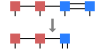
\includegraphics[scale=1.5]{figures/contraction_reseau}
  \end{center}
  \caption[Contraction de deux tenseurs]{
    La contraction de deux tenseurs d'un réseau.
    Cette contraction des tenseurs jaunes en bas à gauche du réseau
    en un nouveau tenseur de rang 3 correspond à l'équation~\eqref{eq:contraction_somme}.
  }
  \label{fig:contraction_reseau}
\end{figure}

Dans les sections~\ref{sec:codes_polaires} et~\ref{sec:codes_polaires_conv},
j'utiliserai plusieurs dizaines voir centaines de tenseurs pour 
représenter des distributions de probabilité.
Dans ce cas, 
la notation de sommation devient inutilisable 
en raison du nombre trop important de tenseurs et d'indices.
Pour contourner ce problème,
j'utiliserai une notation graphique pour les tenseurs.
C'est cette représentation graphique qui porte le nom de réseaux de tenseurs.

Un réseau de tenseur est défini par un graphe $G = (\tenseurs, \aretes)$\footnote{Je fais 
un rappel des notions de théorie des graphes à l'annexe~\ref{chap:theo_graphe}.} où $\tenseurs$ 
est un ensemble de tenseurs et $\aretes \subseteq (\tenseurs \times \tenseurs) \cup \tilde{\tenseurs}$ 
est un ensemble d'arêtes fermées, $\tenseurs \times \tenseurs$, reliant deux tenseurs 
et d'arêtes ouvertes, $\tilde \tenseurs = \qty{\qty{T} : T \in \tenseurs}$, comprenant un seul tenseur.
Une arête $a \in \aretes$ est connectée à un tenseur $T \in \tenseurs$ si $T \in a$.
Le rang d'un tenseur $T \in \tenseurs$ correspond au degré de $T$ dans $G$,
soit le nombre d'arêtes connectées à $T$.
Ainsi, chaque arête connectée à $T$ correspond à un indice de $T$.

Une arête fermée correspond à un indice commun entre deux tenseurs à contracter.
Suite à la contraction d'un indice commun, le réseau est modifié comme 
illustré à la figure~\ref{fig:contraction_reseau}.
Lors de la contraction d'une paire de tenseurs dans un réseau,
le nombre d'arêtes ouvertes du réseau est conservé.
La contraction d'un réseau de tenseurs est ainsi une séquence de contractions 
de paires de tenseurs jusqu'à ce qu'il ne reste qu'un seul tenseur avec des arêtes ouvertes.
Pour ce faire, 
il est important de considéré l'ordre des contractions pour minimiser la taille 
des tenseurs intermédiaires puisque cela peut avoir un impact considérable sur la mémoire
requise et le temps de calcul.
En effet,
il est possible que ces deux quantités augmentent exponentiellement avec le nombre 
de tenseurs et d'arêtes dans le réseau initial.
Trouver l'ordre de contraction optimal est un problème appartenent 
à la classe de complexité $\sharp P$\footnote{Je fais un rappel des notions de la 
théorie de la complexité à l'annexe~\ref{chap:complexite_calcul}. Dans ce cas, 
il est suffisant de comprendre qu'il s'agit d'un problème très difficile même 
en utilisant une grande quantité de ressources numériques.}~\cite{biamonte_tensor_2015}. 
Heureusement,
pour les codes polaires et les codes polaires convolutifs,
un ordre de contraction efficace se présente naturellement.


\section{Codes polaires}
\label{sec:codes_polaires}


C'est en 2009 que Arikan introduit les codes polaires~\cite{arikan_channel_2009}.
Le concept fondamentale derrière la construction des codes polaires est la polarisation
des canaux bruités.
Cette technique permet de convertir deux canaux bruités similaires en un canal moins bruité
et un canal plus bruité.
Ainsi,
un ensemble de canaux presque sans bruit et un ensemble presque inutilisable
sont obtenues en répétant itérativement cette approche à partir de plusieurs canaux similaires.
Ce qui est remarquable est que la fraction de canaux de faible bruit créés ainsi
tend vers la capacité des canaux initiaux.
En combinant cela au fait qu'il existe un algorithme efficace de décodage des codes polaires,
nous obtenons une famille de codes aux performances très prometteuse.
Dans le reste de cette section,
je vais d'abord introduire le procéssus de polarisation des canaux
avant d'introduire la construction des codes polaires
et de finalement présenter l'algorithme de décodage par réseaux de tenseurs. 

\subsection{Polarisation des canaux}

Je vais décrire un canal à partir de sa fonction de poids. 
Ainsi,
le canal binaire symétrique $\canal_p$ est représenté par la fonction de poids
\begin{equation}
  W(y|x) =
  \begin{cases}
    1 - p & \text{si } x = y,\\
    p & \text{si } x \neq y.\\
  \end{cases}
\end{equation}
Cette fonction représente la probabilité de recevoir $y$ si $x$ a été transmis.

Pour la construction des codes polaires,
des canaux plus généraux $W(\vb y | x)$,
où $\vb y \in \qty{0, 1}^m$ est un vecteur de $m$ bits,
sont considérés.
De plus, 
l'analyse se limite aux canaux composés de canaux binaires symétriques.
Dans ce cas, l'information mutuelle d'un canal décrit par $W(\vb y | x)$
est maximisée par une probabilité uniforme des valeurs de $x$.
La capacité est alors~\footnote{
  Sauf indication contraire, les logarithmes dans cette thèse sont calculés en base 2.
}
\begin{align}
  \capacite(W) 
  = I(X ; Y)
  &= \sum_{\vb y \in \qty{0, 1}^m}\sum_{x \in \qty{0, 1}} 
  \Pr(x, y) \log\qty(\frac{\Pr(x, y)}{\Pr(x) \Pr(y)})\notag\\
  &= \sum_{\vb y \in \qty{0, 1}^m}\sum_{x \in \qty{0, 1}} 
  \frac{1}{2}W(\vb y | x) \log\qty(\frac{2 W(\vb y | x)}{W(\vb y | 0) + W(\vb y | 1)})
  \label{eq:capacite_symetrique}
\end{align}
puisque $\Pr(x = 0) = \Pr(x = 1) = 1/2$.

La première étape de la polarisation est de combiner 
deux copies du canal binaire symétrique $W_1$ en un nouveau canal à 2 bits selon 
\begin{equation}
  W_2(\vb y_1^2 | \vb u_1^2) = W_1(y_2 | u_2) W_1(y_1 | u_1 + u_2),
\end{equation}
comme illustré à la figure~\ref{fig:polarisation}.
Dans cette section, je suis la littérature sur la correction d'erreurs
classique et j'utilise la notation $\vb x_i^j = (x_i, x_{i + 1}, \ldots x_j)$.
Le canal $W_2$ est obtenu en transformant l'entrée $(u_1, u_2)$ vers $(u_1 + u_2, u_2)$.
Cette transformation est l'analogue classique de la porte logique CNOT très utilisée 
en informatique quantique.

\begin{figure}[t]
  \begin{center}
    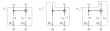
\includegraphics[scale=1.2]{figures/polarisation.pdf}
  \end{center}
  \caption[Polarisation des canaux]{
    Polarisation d'une paire de canaux.
    Le canal $W_2$ est obtenu en combinant deux canaux $W_1$ à l'aide de la porte CNOT.
    Le canal $W_2^{(1)}$ est obtenu en transmettant $u_1$ via $W_2$ lorsque $u_2$ est inconnu.
    Le canal $W_2^{(2)}$ est obtenu en transmettant $u_2$ via $W_2$ lorsque $u'_1$ est connu.
.  }
  \label{fig:polarisation}
\end{figure}

Comme de l'information sur le bit $u_2$ est transmise via les deux canaux initiaux et 
que seule de l'information partielle est transmise sur $u_1$ par le premier canal,
il est intuitif de croire que le bit $u_2$ sera mieux protégé des erreurs. 
C'est cet intuition que je vais maintenant formaliser.

Le canal $W_2$ est décomposé en un mauvais canal $W_2^{(1)}$ et un bon canal $W_2^{(2)}$.
Pour ce faire,
les bits $u_1$ et $u_2$ sont transmis de façon successive.
D'abord, 
le bit $u_1$ est transmis en ignorant la valeur de $u_2$. 
Le mauvais canal,
\begin{equation}
  W_2^{(1)}(\vb y_1^2 | u_1) 
  = \sum_{u_2 \in \qty{0, 1}} W_2(\vb y_1^2 | u_1^2) 
  = \frac{1}{2}\sum_{u_2 \in \qty{0, 1}} W_1(y_2 | u_2) W_1(y_1 | u_1 + u_2),
\end{equation}
est obtenu en supposant qu'il est équiprobable que $u_2 = 0$ et $u_2 = 1$.

Pour retrouver la valeur de $u_1$ transmise par ce canal, 
la valeur de $u_2$ est estimée selon $W_1(y_2 | u_2)$. 
La probabilité de succès est de $1 - p$. 
Ensuite, 
la valeur de $u_1$ est estimée selon $W(y_1 | u_1 + u_2)$.
En supposant la bonne valeur de $u_2$, 
la probabilité de succès de cette étape est également de $1 - p$.
Ainsi, la probabilité totale de succès est de $(1 - p)^2$,
ce qui est inférieure à la probabilité de succès $1 - p$ de $W$.

\begin{figure}
  \begin{center}
    \includegraphics{figures/capacite_polarisation.pdf}
  \end{center}
  \caption[Capacité des canaux polarisés]{Comparaison de la capacité des canaux polarisés.}
  \label{fig:capacite_polarisation}
\end{figure}

Le bon canal est construit en supposant que la valeur de $u_1$ est connue,
soit parce qu'elle est fixée initialement ou qu'elle a été retrouvée avec succès
après l'utilisation du mauvais canal.
La fonction de poids du bon canal est alors
\begin{equation}
  W_2^{(2)}(\vb y_1^2, u'_1 | u_2) 
  = W_1(y_2 | u_2) W_1(y_1 | u'_1 + u_2),
\end{equation}
où la valeur $u'_1$ est connue. 
Dans le cas où $u_1 = 0$, 
utiliser ce canal est équivalent à envoyer deux copies de $u_2$. 
Ainsi, 
s'il y a une seule erreur, alors $y_1 \neq y_2$ et il est possible de détecter l'erreur.
Une erreur doit donc affecter chacun des bits pour que celle-ci ne soit pas détecter.
Cela a une probabilité $p^2$ ce qui est inférieure à la probabilité d'échec $p$ du canal $W_1$.
Une logique similaire s'applique lorsque $u_1 = 1$.

La capacité des différents canaux est calculée à partir 
de l'équation~\eqref{eq:capacite_symetrique}
et est illustrée à la figure~\ref{fig:capacite_polarisation}.
À l'exception des cas où la correction d'erreurs est inutile,
soit lorsque $p = 0$, $p =0.5$ ou $p = 1$,
il est clair, selon la figure, qu'il y a un avantage a utilise le bon canal $W_2^{(2)}$.
Par exemple, pour $p = 0.2$, la capacité de celui-ci est près du double 
de la capacité initiale et plus de 4 fois supérieure à la capacitié du mauvais canal $W_2^{(1)}$.

\subsection{Construction des codes polaires}

L'astuce derrière la construction des codes polaires est de repéter itérativement le 
processus de polarisation des canaux.
En effet, 
en répérant cet opération sur deux bons canaux obtenus par polarisation,
nous obtenons un nouveau canal encore plus performant et un canal de qualité moyenne.
De même,
en polarisant deux mauvais canaux, nous obtenons un canal de qualité moyenne et 
un canal médiocre.
En répétant ce procédé un très grand nombre de fois,
Arikan a montré~\cite{arikan_channel_2009} 
que la fraction des canaux atteignant une capacité de 1
tend vers $1 - H_2(p)$, soit la capacité des canaux initiaux.
L'idée est alors d'utiliser ces canaux pour transmettre l'information
et fixer la valeur des autres bits à 0.

\begin{figure}
  \begin{center}
    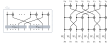
\includegraphics[scale=1.3]{figures/circuit_code_polaire.pdf}
  \end{center}
  \caption[Circuit des codes polaires]{
    Circuit d'encodage pour les codes polaires.
    À gauche, la relation de récurrence pour ajouter un niveau de polarisation.
    À droite, la transmission de 8 bits encodés à l'aide de trois niveaux de polarisation.
  }
  \label{fig:circuit_code_polaire}
\end{figure}

De façon similaire à la polarisation d'une paire de canaux,
la polarisation de $n = 2^m$ canaux s'effectue en combinant
d'abord les $n$ canaux $W_1$ en un seul canal,
\begin{equation}
  W_n(\vb y_1^n | \vb u_1^n) = \prod_{i=0}^n W_1(y_i | x_i),
\end{equation}
où $\vb x_1^n = C_n \cdot \vb u_1^n$.
Le circuit d'encodage $C_n$ est obtenu de manière récursive à partir de la relation illustrée
à la figure~\ref{fig:circuit_code_polaire} et en considérant $C_1$ comme le circuit identité
sur un seul bit.

Par la suite,
le canal $W_N$ est décomposé en une série de canaux,
\begin{equation}
  W_n^{(i)}(\vb y_1^n, \vb u_1^{i - 1} | u_i) 
  = \frac{1}{2^{n - i}}
  \sum_{u_{i+1}^n \in \qty{0, 1}^{n - i}} W_n(\vb y_1^n | \vb u_1^n),
\end{equation}
permettant la transmission d'un bit.
Ainsi, 
le bit $u_i$ est transmis en connaissant la valeur des bits précédents et en 
ignorant la valeur des bits suivants de probabilité uniforme.
Il reste alors à trouver l'ensemble des canaux ayant les plus grandes capacités
et de fixer la valeur des autres bits à 0.
Cela engendre un protocole de communication permettant d'envoyer $k \to n(1 - H_2(p))$
encodés à l'aide de $n = 2^m$ bits, ce qui est optimal pour le 
canal binaire symétrique.

Il est évident que le bit $u_n$ est le mieux protégé puisqu'il se retrouve
toujours du bon côté de la polarisation. 
De même, 
le bit $u_1$ est le plus bruyant, car il est toujours du mauvais côté.
Cependant, 
il est plus difficile d'ordonner les bits centraux qui se retrouve parfois du bon côté
et parfois du mauvais.
Il est tentant d'essayer de calculer la capacité de chaque canaux et des les ordonnées
ainsi, mais ce calcul implique la somme de $2^n$ termes pour chacun des canaux. 
Il est alors impossible de faire ce calcul en un temps raisonnable.
Il existe quelques façons de contourner ce problème.
D'abord Arikan~\cite{arikan_channel_2009} propose d'utiliser le paramètre de Bhattacharyya,
\begin{equation}
  Z(W) = \sum_{\vb y} \sqrt{W(\vb y|0)W(\vb y|1)},
\end{equation}
qui est relié à la capacité par
\begin{equation}
  \log\qty( \frac{2}{1 + Z(W)} )
  \leq  
  \capacite(W) 
  \leq 
  \sqrt{1 - Z(W)^2} .
\end{equation}
L'avantage du paramètre de Bhattacharyya est qu'il existe un algorithme récursif pour
calculer sa valeur pour l'ensemble des canaux en temps polynomial.

Dans l'article associé à cette thèse, 
je présente une autre approche plus simple, 
mais un peu moins précise, 
pour choisir les canaux.
Pour la suite, 
je vais définir un code polaire en fonction du nombre de niveaux de polarisation $m$
et d'un ensemble de bits $\mathcal F$ dont la valeur est fixée à 0.


\subsection{Décodage par réseaux de tenseurs}

\begin{figure}
  \begin{center}
    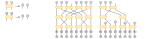
\includegraphics[scale=1.3]{figures/decodage_codes_polaires.pdf}
  \end{center}
  \caption[Circuit des codes polaires]{
    Circuit d'encodage pour les codes polaires.
    À gauche, la relation de récurrence pour ajouter un niveau de polarisation.
    À droite, la transmission de 8 bits encodés à l'aide de trois niveaux de polarisation.
  }
  \label{fig:decodage_codes_polaires}
\end{figure}

\section{Codes polaires convolutifs}
\label{sec:codes_polaires_conv}

\section{Comparaison de la profondeur et de la largeur des codes polaires convolutifs}

Dans celui-ci,
nous comparons plusieurs généralisations des codes polaires basées sur la construction 
des codes polaires convolutifs CITATION DAVID ET ANDREW.
Ces généralisations varient la largeur des codes polaires en utilisant des portes 
de polarisation à plus de 2 qubits 
et varient la profondeur en ajoutant des couches convolutives 
de portes de polarisation à chaque niveau.
Ces deux modifications ne changent la complexité que par un facteur multiplicatif constant.

Le résultat principal de l'article est qu'augmenter la largeur des codes 
nuit aux performances alors qu'augmenter la profondeur augmente les performances.
Lorsque le nombre d'opérations nécessaires au décodage est pris en compte,
il est optimal de choisir une largeur et une profondeur de 2.

\subsection{Motivation du projet}

\subsection{Résultat principal}

\subsection{Article}
Cet article ayant pour titre original \textit{Depth versus Breadth in Convolutional Polar Codes}
a été publié en 2018 dans la cadre de la conférence \textit{IEEE Information Theory Workshop}.



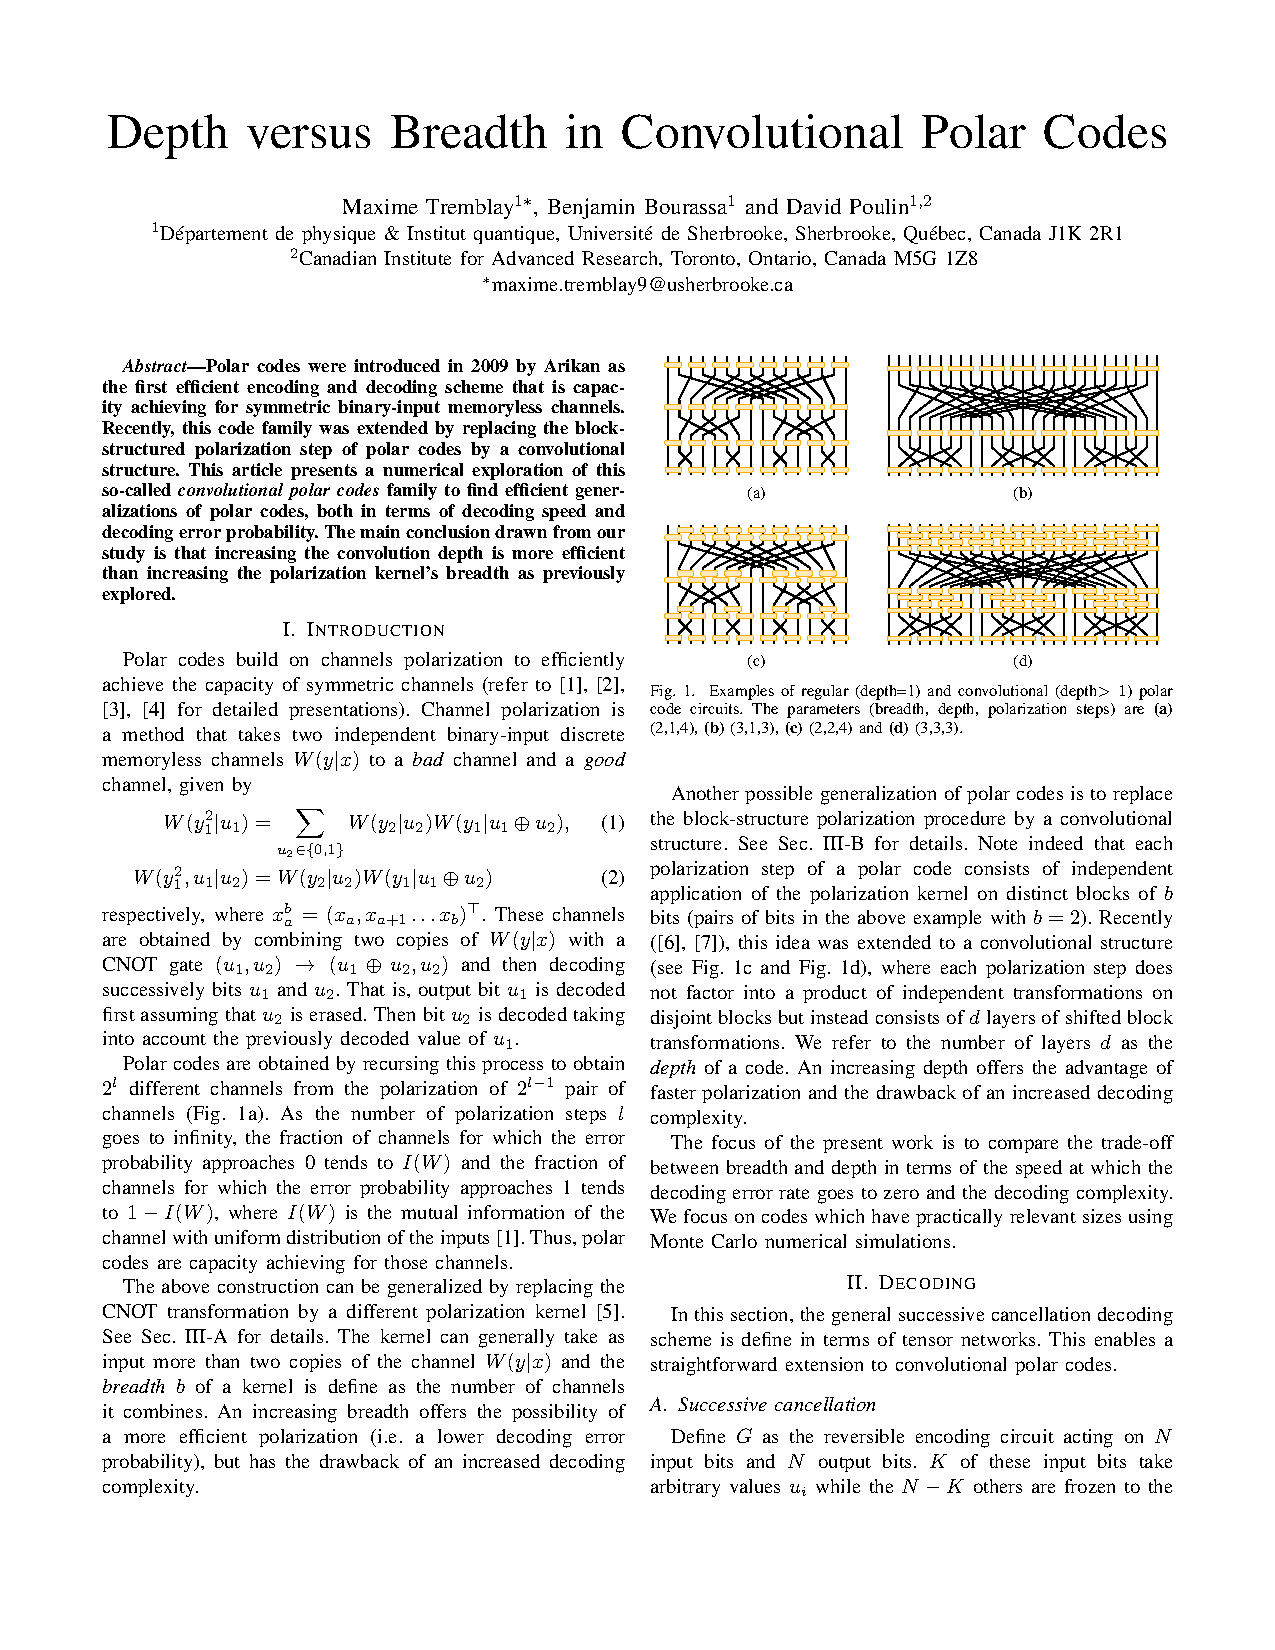
\includepdf[pages=-]{articles/conv_polar_codes.pdf}


\begin{comment}
\end{comment}

\chapter{Construction de codes correcteurs quantiques}

Dans le chapitre précédent, 
je me suis intéressé à la correction des erreurs lors de la communication classique.
Pour la suite de la thèse,
je quitterai ce régime pour m'intéresser au régime quantique.
Dans ce chapitre, 
je m'intéresserai plus particulièrement à la protection de l'information 
dans un modèle quantique simplifié avant de présenter la conception d'une mémoire 
quantique au prochain chapitre.
Ce modèle simplifié ressemble au canal binaire symétrique présenté au premier chapitre
et il permet d'étudier la construction de codes correcteurs d'erreurs quantiques sans prendre en compte les détails d'implémentation.

De façon semblable au scénario classique,
concevoir des codes correcteurs qui permettent de bien protéger l'information avec un nombre raisonnable de qubits supplémentaires est crucial.
En fait,
la présence des erreurs est l'un des obstacles parmi les plus
limitants pour la réalisation de calculs quantiques.
Ainsi, 
la correction d'erreurs ne se limite pas à des scénarios de communication 
comme dans le cas classique,
mais sera omniprésente dans un système de calcul quantique.

Cette importance accrue des erreurs dans les systèmes quantiques s'explique
principalement du fait qu'il s'agit de systèmes analogues plutôt que digitaux.
Un système est digital lorsque chacun de ses éléments peut prendre un nombre fini
de valeurs. 
Dans le cas des ordinateurs classiques,
chaque bit prend soit la valeur 0 ou la valeur 1.
Ainsi,
une quantité continue comme une différence de potentiel représente physiquement un bit tout en le protégeant des erreurs.
Par exemple,
le bit 0 peut être associé à une valeur de 0 volt et le bit 1 à une valeur de 5 volts.
Dans le cas où une valeur de 4.9 volts serait mesurée, il est fort probable que 
la valeur désirée était le bit 1.
Donc, en absence des perturbations externes présentent lors de la communication,
l'information classique est relativement robuste.

Au contraire, un système quantique est analogue puisqu'il existe une infinité d'états accessibles.
Par exemple, toutes paires de nombres complexes $a$ et $b$ telles que $a^2 + b^2 = 1$
représentent l'état d'un qubit.
Ainsi, 
une faible variation de ces paramètres représente un état différent
et distinguer l'état désiré d'un état corrompu est généralement impossible.
De plus, l'accumulation de ces petites différences peut complètement
changer le résultat d'un calcul.

Ces erreurs émergent généralement de processus de décohérence.
Par exemple,
un système quantique dans un état excité tend naturellement à retourner dans un état de moindre énergie.
Au milieu des années 1990,
plusieurs scientifiques croyaient que
les erreurs engendrées par la décohérence des systèmes quantiques
représentaient un obstacle insurmontable au calcul quantique~\cite{unruh_maintaining_1995, palma_quantum_1996, landauer_is_1995, chuang_quantum_1995}.
Leurs arguments reposaient entre autres sur le théorème de non-clonage~\cite{wootters_single_1982}
stipulant qu'il est impossible de copier l'état d'un qubit vers un second qubit.
Cela semblait donc empêcher l'utilisation de la redondance pour 
protéger le système des erreurs comme c'est le cas pour la communication classique.

Nous savons aujourd'hui comment contourner ces limitations. 
Les premiers à avoir proposé une solution sont Calderbank, Shor et Steane~\cite{calderbank_good_1996, steane_multiple-particle_nodate}.
D'ailleurs, à la prochaine section,
je vais introduire une importante famille de codes correcteurs quantiques, les codes CSS, qui porte leur nom.
En réponse à ce résultat, Gottesman~\cite{gottesman_stabilizer_1997} a introduit le formalisme des codes stabilisateurs
que je vais utiliser dans ce chapitre pour décrire les codes correcteurs quantiques.

Depuis,
plusieurs familles de codes correcteurs quantiques ont été introduites.
Les codes les plus étudiés sont sans aucun doute les codes de surfaces et 
les codes toriques introduits par Kitaev~\cite{kitaev_fault-tolerant_2003}.
Cependant,
ces codes, bien qu'excellent pour protéger le système,
ne permettent pas d'encoder efficacement un grand nombre de qubits~\cite{bravyi_tradeoffs_2010}.
Pour contrer ce problème,
les codes quantiques d'opérateurs de parité à faible 
densité~(LDPC, de l'anglais \textit{low-density parity-check})
reçoivent de plus en plus d'attention.
Cet intérêt est en partie stimuler par le succès des codes LDPC classiques introduits
par Gallager~\cite{gallager_low-density_1962}.
De plus, il a été montré par Gottesman~\cite{gottesman_fault-tolerant_2013}
qu'il est possible d'utiliser des codes quantiques LDPC pour 
construire des ordinateurs quantiques protégés des erreurs avec 
un surcout constant en qubits.
Il s'agit donc d'outils importants pour la réalisation du calcul quantique à grande échelle.

Les codes quantiques LDPC incluent plusieurs familles,
dont les codes par produit d'hypergraphes~\cite{tillich_quantum_2014}
et les codes par produit homologique~\cite{bravyi_homological_2014}.
Comme l'indique le nom de ces exemples,
les codes quantiques LDPC sont généralement obtenus par le produit 
de structures associées à des codes correcteurs classiques.
Dans le cadre de cette thèse,
j'ai conçu une approche qui permet plutôt de générer des codes correcteurs quantiques
directement,
sans avoir recours à une construction classique au préalable.
L'un des principaux avantages de cette méthode est sa flexibilité 
lors de la construction des codes.
En fait,
cette construction permet de générer n'importe quelle famille de codes stabilisateurs,
dont les codes LDPC.

Cette approche repose sur la résolution d'un problème de satisfaction de contraintes.
Bien que ce problème soit généralement difficile à résoudre,
j'ai numériquement identifié des régimes pour lesquels il est aisé de
construire des codes correcteurs quantiques
et des régimes pour lesquels la tâche est beaucoup plus ardue.
Cela, bien que surprenant, est un comportement attendu pour ce type de problème.

Je reviendrai sur cela après avoir présenté le formaliste des canaux bruités quantiques 
et des codes stabilisateurs.
Finalement,
je présenterai l'article expliquant la construction et 
mettant de l'avant les résultats de ce projet.

\section{Correction d'erreurs quantique}

\subsection{Canaux bruités quantiques}

Un état quantique est généralement représenté par un opérateur de densité $\rho$
de trace unité.
Une évolution arbitraire d'un état $\rho$ vers un état $\rho'$
c'est-à-dire une combinaison d'opérations unitaires,
de mesures et d'interactions avec l'environnement, 
est représentée par une application
\begin{align}
  \rho' = \mathcal{E}(\rho).
\end{align}
Pour décrire plus précisément cette transformation,
j'utiliserai les opérateurs de Krauss.
Dans ce cas,
l'application est définie par
\begin{align}
  \mathcal{E}(\rho) = \sum_{k} E_k \rho E_k^\dag,
\end{align}
avec la condition que 
\begin{align}
  \sum_k E_k^\dag E_k = I.
\end{align}
Cette dernière permet d'assurer que $\tr(\mathcal{E}(\rho)) = 1$.

Dans leur excellent livre d'introduction à l'informatique quantique de 
Neilsen et Chuang~\cite{nielsen_quantum_2010} motivent en détail 
cette définition générale pour l'évolution d'un état quantique.
Ainsi, je me limite à une justification intuitive de cette définition
et j'invite les personnes intéressées à consulter le huitième chapitre de ce livre.

De façon générale,
l'état $\rho$ évolue au sein d'un environnement dont les états de base 
sont $\qty{\ket{e_0}, \ket{e_1}, \ldots}$.
Au début d'une expérience (ou d'un calcul),
le système et l'environnement sont dans un état de produit tensoriel,
soit un état sans intrication.
De plus, il est suffisant de considérer que l'environnement est dans l'état 
pur $\ket{e_0}$.
En effet,
si ce n'est pas le cas, il suffit de choisir un environnement plus grand jusqu'à 
obtenir un état pur.
Ainsi,
l'état initial du système et de l'environnement est $\rho \otimes \op{e_0}$.

\begin{figure}
  \begin{center}
    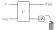
\includegraphics{figures/circuit_canal_quantique.pdf}
  \end{center}
  \caption[Représentation en circuit d'un canal quantique]{
    Représentation en circuit d'un canal quantique.
    Le résultat de la mesure est ignoré.
  }
  \label{fig:circuit_canal_quantique}
\end{figure}

Par la suite,
un opérateur unitaire $U$ est appliqué sur le système et l'environnement,
suivi d'une mesure de l'environnement sans connaitre le résultat.
Le circuit correspondant est illustré à la figure~\ref{fig:circuit_canal_quantique}.
Ainsi, l'état final du système est
\begin{equation}
  \mathcal{E}(\rho) 
  = \tr_{\text{env}}\qty(U(\rho \otimes \op{e_0})U^\dag)
  = \sum_k \bra{e_k}U(\rho \otimes \op{e_0}) U^\dag \ket{e_k}
  = \sum_k E_k \rho E_k^\dag
\end{equation}
avec $E_k = \mel{e_k}{U}{e_0}$.
Alors,
l'application $\mathcal{E}$ représente la transformation de l'état d'un système quantique
lorsque celui-ci interagit avec son environnement et que l'on ignore l'état final
de l'environnement.

Une autre interprétation est qu'à la suite de l'application $\mathcal E$,
le système se retrouve dans l'état $\rho_k \propto E_k \rho E_k^\dag$
avec probabilité $p_k = \tr(E_k \rho E_k^\dag)$.
Il est alors possible d'écrire l'application selon
\begin{align}
  \mathcal E(\rho) = \sum_k p_k \rho_k.
\end{align}
Cette formulation montre clairement l'utilité de $\mathcal E$ pour
représenter un canal bruité quantique.
De façon comparable au canal bruité classique,
un canal quantique transforme un premier état 
vers un second état choisi aléatoirement.

Dans cette thèse,
je me limite aux canaux bruités quantiques avec des opérateurs 
de Krauss $E_k$ proportionnels aux opérateurs de Pauli.
Les opérateurs de Pauli pour un seul qubit sont 
\begin{align}
  &I = \op{0}{0} + \op{1}{1}, 
  &&Y = -i\op{0}{1} + i\op{1}{0}, \notag \\
  &X = \op{0}{1} + \op{1}{0}, 
  &&Z = \op{0}{0} - \op{1}{1}.
\end{align}
Le groupe~\footnote{Je fais un rappel des notions de théorie des groupes à l'annexe~\ref{chap:theo_groupes}}
de Pauli $\mathcal P_n$ de $n$ qubits est un groupe multiplicatif sur 
l'ensemble des opérateurs $\qty{I, X, Y, Z}^n$ avec une phase parmi $\qty{1, i, -1, -i}$.
Dans ce cas,
le canal s'écrit généralement comme
\begin{align}
  \mathcal E(\rho) = \sum_{P \in \mathcal P_n} p_P P\rho P.
\end{align}
Le poids $|P|$ d'un opérateur de Pauli $P$ est le nombre d'opérateurs différent de $I$ qui le compose.
Par exemple, $|i\cdot XIYX| = 3$.
Pour l'ensemble des canaux que je considèrerai,
la probabilité d'une erreur $P \in \mathcal P_n$ diminue exponentiellement avec le poids 
de celle-ci.

De prime abord,
cette approche semble limitée,
mais puisque les opérateurs de Pauli forment une base,
il est possible de représenter un opérateur de Krauss
comme une combinaison linéaire de ces derniers.
Ainsi,
un protocole qui permet de protéger un système quantique contre les erreurs 
$Q \subseteq \mathcal P_n$ protège également le système contre toutes les 
combinaisons linéaires des opérateurs de $Q$~\cite{knill_theory_1997}.
Ce modèle est donc suffisant pour construire une théorie générale de la correction d'erreurs quantique.

En particulier,
dans l'article de ce chapitre,
j'utilise le canal d'effacement quantique pour évaluer la performance
des codes correcteurs que je construis.
Ce canal représente la situation où l'information contenue dans certains qubits,
dont on connait la position, est complètement perdue.
On dit alors que ces qubits sont effacés.
En laboratoire, cela correspond par exemple à la défaillance d'une composante électronique
ou à la perte d'un photon.
Pour représenter cette situation, l'état $\rho$ est associé à un second registre
permettant de marquer les qubits effacés.
Dans le cas d'un seul qubit avec une probabilité d'effacement $p$,
le canal s'écrit
\begin{equation}
  \mathcal E_p(\rho \times \op{0}) 
  = (1 - p) \rho \otimes \op{0} + p \frac{I}{2} \otimes \op{1}.
\end{equation}
Dans cet équation,
l'opérateur $I/2$ est utilisé pour représenter un état maximalement mixé
sans aucune information sur l'état initial $\rho$.
Le second registre indique la présence de l'effacement.
Comme 
\begin{align}
  I = \frac{1}{2} \qty(
  I\rho I + X \rho X + Y \rho Y + Z \rho Z
)
\end{align}
pour tout opérateur $\rho$\footnote{
  En notant $f(\rho) = I\rho I + X\rho X + Y \rho Y + Z \rho Z$,
  on remarque que $f(I/2) = I$ et que $f(X) = f(Y) = f(Z) = 0$.
  De plus,
  pour avoir une trace unité,
  une matrice densité se décompose comme $\rho = I/2 + aX + bY + cZ$,
  ce qui permet de conclure.
},
il est possible de réécrire le canal à l'aide d'opérateurs de Pauli à 2 qubits.
Ainsi,
\begin{equation}
  \mathcal E_p(\rho \times \op{0}) 
  = \qty(1 -  p) \rho \otimes \op{0} + \frac{p}{4} \qty(\rho + X \rho X + Y \rho Y + Z \rho Z)\otimes \qty(X\op{0}X).
\end{equation}

Dans l'article,
je présente plus en détail le canal d'effacement.
Entre autres,
je généralise le canal au cas à plusieurs qubits
en plus de présenter un algorithme de décodage optimal applicable à n'importe quel
code correcteur quantique pour ce canal.
Ce décodeur universel est la raison principale pour utiliser le canal d'effacement.
Celui-ci permet d'étudier de nouveaux codes sans nécessairement avoir besoin de construire des 
décodeurs spécialisés pour des canaux bruités plus complexes~(voir par exemple \cite{pastawski_holographic_2015, gullans_quantum_2021}).

Dans le chapitre suivant,
j'utiliserai un modèle de bruit plus réaliste qui permet
de représenter une mémoire quantique.
Celui-ci est également construit à partir d'opérateurs de Krauss proportionnels à des
opérateurs de Pauli.

\subsection{Codes stabilisateurs}

L'une des meilleures ressources pour une présentation complète du formalisme des codes
stabilisateurs est la thèse de doctorat de Gottesman~\cite{gottesman_stabilizer_1997}.
Dans cette section,
je me limiterai plutôt aux concepts essentiels à la compréhension des travaux et de l'article.

De façon comparable aux codes classiques,
les codes correcteurs quantiques encodent les états d'un espace de Hilbert
dans un sous-espace d'un espace de plus grande dimension.
Dans le cas des qubits,
les états de l'espace de Hilbert $\mathcal H_2^k$ sont encodés à l'aide d'un
sous-espace $\code \subseteq \mathcal H_2^n$.
Pour préserver la linéarité de la mécanique quantique,
le code $\code$ doit être un espace linéaire.
Ainsi,
si $\ket\psi, \ket\phi \in \code$,
alors $\alpha\ket\psi + \beta\ket\phi \in \code$ 
pour toutes paires $\alpha, \beta$ de nombres complexes.~\footnote{
  Pour simplifier la présentation,
  je laisse tomber la normalisation des états quantiques.
}

Un exemple de code quantique permettant d'encoder un qubit à l'aide de neuf qubits est 
le code de Shor~\cite{shor_scheme_1995} défini par l'encodage
\begin{align}
  \ket{0} \to \ket{\bar{0}} = (\ket{000} + \ket{111}) \otimes (\ket{000} + \ket{111}) \otimes (\ket{000} + \ket{111}), \notag \\
  \ket{1} \to \ket{\bar{1}} = (\ket{000} - \ket{111}) \otimes (\ket{000} - \ket{111}) \otimes (\ket{000} - \ket{111}).
  \label{eq:code_shor}
\end{align}
Par linéarité, l'état $\alpha \ket{0} + \beta \ket{1}$ est encodé avec l'état 
$\alpha \ket{\bar{0}} + \beta\ket{\bar {1}}$.
Je ne détaillerai pas ce code,
mais celui-ci illustre qu'il n'est pas pratique d'énumérer l'encodage des états de base
pour définir un code.
D'abord,
l'espace $\mathcal H_2^k$ requiert $2^k$ états de base
et chacun de ceux-ci implique une superposition de $\mathcal O(2^n)$ 
si le code $\code$ est un sous-espace de l'espace de Hilbert à $n$ qubits.

Le formalisme des stabilisateurs permet de contourner ce problème en offrant une 
représentation beaucoup plus efficiente de certains états quantiques.
D'abord,
un état $\ket\phi$ est stabilisé par l'opérateur $U$ lorsque $U\ket\psi = \ket\psi$,
soit lorsque $\ket \phi$ est un état propre de valeur propre $+1$ de $U$.
Un état ou un sous-espace est alors représenté par les opérateurs qui le stabilisent.
Par exemple,
l'état $\ket{00} + \ket{11}$ est l'unique état à deux qubits stabilisé par 
les opérateurs $XX$ et $ZZ$. 
De même,
les états $\ket 00$ et $\ket 11$ forment une base
pour les états stabilisés par l'opérateur $ZZ$.
Il est important de choisir des opérateurs qui commutent pour assurer 
que ceux-ci partagent les mêmes états propres.
De plus, l'opérateur identité $I$ stabilise tous les états
et l'opérateur $-I$ ne stabilise aucun état.

De façon plus générale,
un groupe stabilisateur $\mathcal S$ pour $n$ qubits est un sous-groupe abélien 
du groupe de Pauli $\mathcal P_n$ excluant l'opérateur $-I$.
Cette exclusion implique également que tous les opérateurs ayant la phase $i$ ou $-i$ sont exclus.
Un code stabilisateur $\code(\mathcal S)$ est alors l'espace des états stabilisés par $\mathcal S$.
De plus,
puisque les états stabilisés par les opérateurs $P, Q \in \mathcal P_n$ sont également
stabilisés par l'opérateur $PQ$,
il est commun de choisir un ensemble de générateurs $g(\mathcal S) = \qty{S_1, \ldots, S_m}$
pour décrire le groupe stabilisateur
\begin{align}
  \mathcal S = 
  \qty{
    \prod_{i=1}^m S_i^{a_i} : \vb a \in \qty{0, 1}^m
  }
\end{align}
de $2^m$ éléments.
Lorsque les générateurs sont indépendants,
c'est-à-dire qu'il n'est pas possible d'en obtenir un comme le produit des autres,
le code $\code(\mathcal S)$ a une dimension $2^{n - m}$.
Ainsi, 
pour encoder $k$ qubits avec un code de $n$ qubits,
exactement $m = n - k$ générateurs indépendants sont nécessaires.

Le code de Shor introduit à l'équation~\eqref{eq:code_shor} est stabilisé
par le groupe généré par les opérateurs 
\begin{gather}
    X_1 X_2 X_3 X_4 X_5 X_6, \quad
    Z_1 Z_2, \quad Z_4 Z_5, \quad Z_7 Z_8, \notag \\
    X_4 X_5 X_6 X_7 X_8 X_9, \quad
    Z_2 Z_3, \quad Z_5 Z_6, \quad Z_8 Z_9.
\end{gather}
Dans ce cas précis,
le formalisme stabilisateur peut sembler légèrement encombrant,
mais il permet généralement de représenter un code de $n$ qubits encodant $k$ qubits
à l'aide de $n - k$ opérateurs de poids $\mathcal O(n)$.
Le cout total de la représentation est alors $\mathcal O(n^2)$, ce qui est un gain exponentiel
par rapport à l'énumération des états de base du code en notation de Dirac.
Pour la suite,
j'utiliserai la notation $[n, k]$ pour représenter un code stabilisateur arbitraire 
encodant l'espace $\mathcal H_2^k$ dans un sous-ensemble $\code \subseteq \mathcal H_2^n$.

Le syndrome d'une erreur $E \in \mathcal P_n$,
qui affectent un état $\ket\psi$ quelconque d'un code $[n, k]$,
est le résultat des mesures des générateurs du groupe stabilisateur.
Puisque les opérateurs de Pauli commutent ou anticommutent,
le résultat de chacune de ces mesures est $+1$ ou $-1$.
En effet, si $SE = \pm ES$ pour un stabilisateur $S$,
alors
\begin{equation}
  SE\ket\psi = \pm E S \ket\psi = \pm E\ket\psi.
\end{equation}
Ainsi,
l'état $E\ket\psi$ est un état propre de valeur propre $\pm 1$ de $S$.
Les composantes du syndrome $\vb{s}(E) \in \qty{+1, -1}^{n - k}$
sont données par la relation $S_iE = s_i S_i E$ pour $S_i \in g(\mathcal S)$.

Il est important de noter que le syndrome est indépendant de l'état $\ket \psi$.
Conséquemment,
une mesure du syndrome permet de détecter la présence d'erreurs sans corrompre l'état du système.
À partir de cette information,
un décodeur essaie de trouver une correction $F$ telle que $FE \in \mathcal S$, 
soit que $FE\ket\psi = \ket\psi$ pour tout état code $\ket\psi$.
Le choix de la correction n'est pas unique, car, si $FE \in \mathcal S$,
alors $(SF)E \in \mathcal S$ pour tous $S \in \mathcal S$.
Ainsi,
toutes corrections $F' = SF$ sont également valides.

Formellement,
tous les opérateurs $P \in \mathcal P_n$ de la même classe du groupe quotient $\mathcal P_n/\mathcal S$
ont le même effet sur le code puisque $P\ket\psi = PS\ket\psi$ pour tout $S \in \mathcal S$.
La classe d'un opérateur $P \in \mathcal P_n$ est l'ensemble $P\cdot \mathcal S = \qty{PS : S\in \mathcal S}$,
soit l'ensemble des opérateurs équivalent après multiplication par un stabilisateur.
De plus,
comme $|\mathcal P_n| = 4^{n+1}$,
le groupe quotient $\mathcal P_n/\mathcal S$ d'un code $[n, k]$ tel que $|\mathcal S| = 2^{n - k}$
possède $2^{n+k+2}$ classes.
En comparaison,
seulement $2^{n-k}$ syndromes sont possibles,
ce qui implique que $2^{2k + 2} = 4^{k + 1}$ classes d'opérateurs ont exactement le même syndrome,
mais des effets différents sur le code.

Les opérateurs appartenant aux classes ayant le syndrome $\qty{+1, +1, \ldots, +1}$
sont des représentations à $n$ qubit des opérateurs de Pauli $\mathcal P_k$
agissant sur le code.
Ces opérateurs forment le groupe des opérateurs logiques $\mathcal L$ et correspondent
au centralisateur,
\begin{align}
  C_{\mathcal P_n}(\mathcal S) 
  = \qty{P \in \mathcal P_n : PS = SP, \forall S \in \mathcal S},
\end{align}
du groupe stabilisateur.
Puisqu'un opérateur logique $L \in \mathcal L$ commute avec l'ensemble des stabilisateurs,
\begin{equation}
  S(L\ket\psi) = LS\ket\psi = L\ket\psi
\end{equation}
pour tout état code.
En conséquence,
$L\ket\psi$ est également un état code.
De façon similaire,
pour un syndrome arbitraire,
les $4^{k+1}$ classes ayant ce syndrome sont reliées par les opérateurs logiques.

On remarque que $\mathcal S \subset \mathcal L$.
En effet, le groupe stabilisateur correspond à l'opérateur $I$ sur le code.
De même, les classes $-\mathcal S$, $i\mathcal S$ et $-i\mathcal S$ correpondent
aux opérateurs $-I$, $iI$ et $-iI$.
La correspondance entre les autres opérateurs logiques et opérateurs de Pauli est
arbitraire tant que les relations de commutations sont respectées.

La conséquence de tout cela est qu'il est possible de décomposer un opérateur
$E \in \mathcal P_n$ en produit $LC$ où $C$ est un opérateur de même syndrome que $E$
et $L$ est un opérateur logique.
Il n'est pas nécessaire que $E = LC$, mais plutôt que $LC$ soit un élément de la classe $E \cdot \mathcal S$.
Cette décomposition permet de construire une procédure de décodage optimale que l'on 
nomme décodeur par maximum de vraissemblance (MV).
À partir du syndrome de l'opérateur $E$, 
le décodeur MV choisi d'abord aléatoirement une correction $C$ de même syndrome avant
de choisir un opérateur logique selon
\begin{align}
  L_{\text{MV}} = \arg\max_{L \in \mathcal L} \sum_{S \in \mathcal S} \Pr[LSC].
\end{align}
L'idée derrière le décodeur MV est qu'il existe un opérateur logique $L^*$ tel que $C = L^*E$.
Alors, le décodage est un succès si $L_{MV}$ et $L^*$ ont la même classe,
c'est-à-dire si $L_{MV}C = SE$ pour un certain stabilisateur $S \in \mathcal S$.
Ainsi, pour tout opérateur logique $L$, nous avons que 
\begin{align}
  \sum_{S\in \mathcal S} \Pr[LSC]
  =
  \sum_{S\in \mathcal S} \Pr[LSL^*E]
  =
  \sum_{S\in \mathcal S} \Pr[LL^*SE].
\end{align}
Dans le cas typique,
le poids de $E$ est faible puisque la probabilité d'un opérateur diminue avec son poid.
Ainsi, la somme est maximisée par $LL^* \in \mathcal S$ si le poids de chacun des opérateurs de
$\mathcal L \setminus \mathcal S$ est élevé.
Sinon,
la somme est maximisée par $LL^* \equiv P \in \mathcal L \setminus \mathcal S$ 
et l'application de cette correction laisse le système avec une erreur $L_{MV}CE = LL^*EE = P$ indectable.

Le décodeur échoue dans deux cas,
soit si le poids de $E$ est élevé, ce qui est hors de notre contrôle,
ou s'il existe un opérateur logique non stabilisateur de faible poids.
Ainsi,
il est important de construire des codes stabilisateurs pour lesquels la distance minimale,
\begin{align}
  d = \min_{L \in \mathcal L \setminus \mathcal S} |L|,
\end{align}
est élevée.
Le décodeur MV permet de corriger toutes les erreurs dont le poids est inférieur à $d / 2$.
Il n'est pas exclus que des erreurs de poids plus élevés soit corrigibles, 
mais les paramètres $n$, $k$ et $d$ d'un code permettent d'estimer rapidement la capacité
de ce dernier à corriger les erreurs en fonction de son rendement $k/n$.

Par contre,
calculer la distance minimale d'un code requiert de comparer le poid d'un nombre exponentiel d'opérateurs.
Il en est de même pour le calcul de $L_{MV}$ qui requiert un nombre exponentiel de compaisons.
Il est donc généralement impossible de calculer ces quantité et des simulations numériques 
doivent être effectuées pour estimer la performance d'un code à l'aide d'un décodeur sous-optimal.
Je reviendrai sur ce point à la section~\ref{sec:seuil_perf} après avoir présenté
les codes de Calderbank-Shor-Steane et une représentation graphique des codes
stabilisateurs aux prochaines sections.

\subsection{Codes CSS}

\subsection{Graphes de Tanner}


\subsection{Théorème du seuil et évaluation de la performance des codes correcteurs quantiques}
\label{sec:seuil_perf}
CITER Gottesman-Knill



\section{Problèmes de satisfaction de contraintes}
\subsection{Transition de phases et seuil de satisfiabilité}

\section{Article : Une multitude de codes stabilisateurs éparses}

Cet article soumis au journal Quantum à l'été 2022 a pour titre original
\textit{Finite-rate quantum sparse codes aplenty}.
Celui-ci était toujours en processus de révision lors de la soumission de cette thèse.

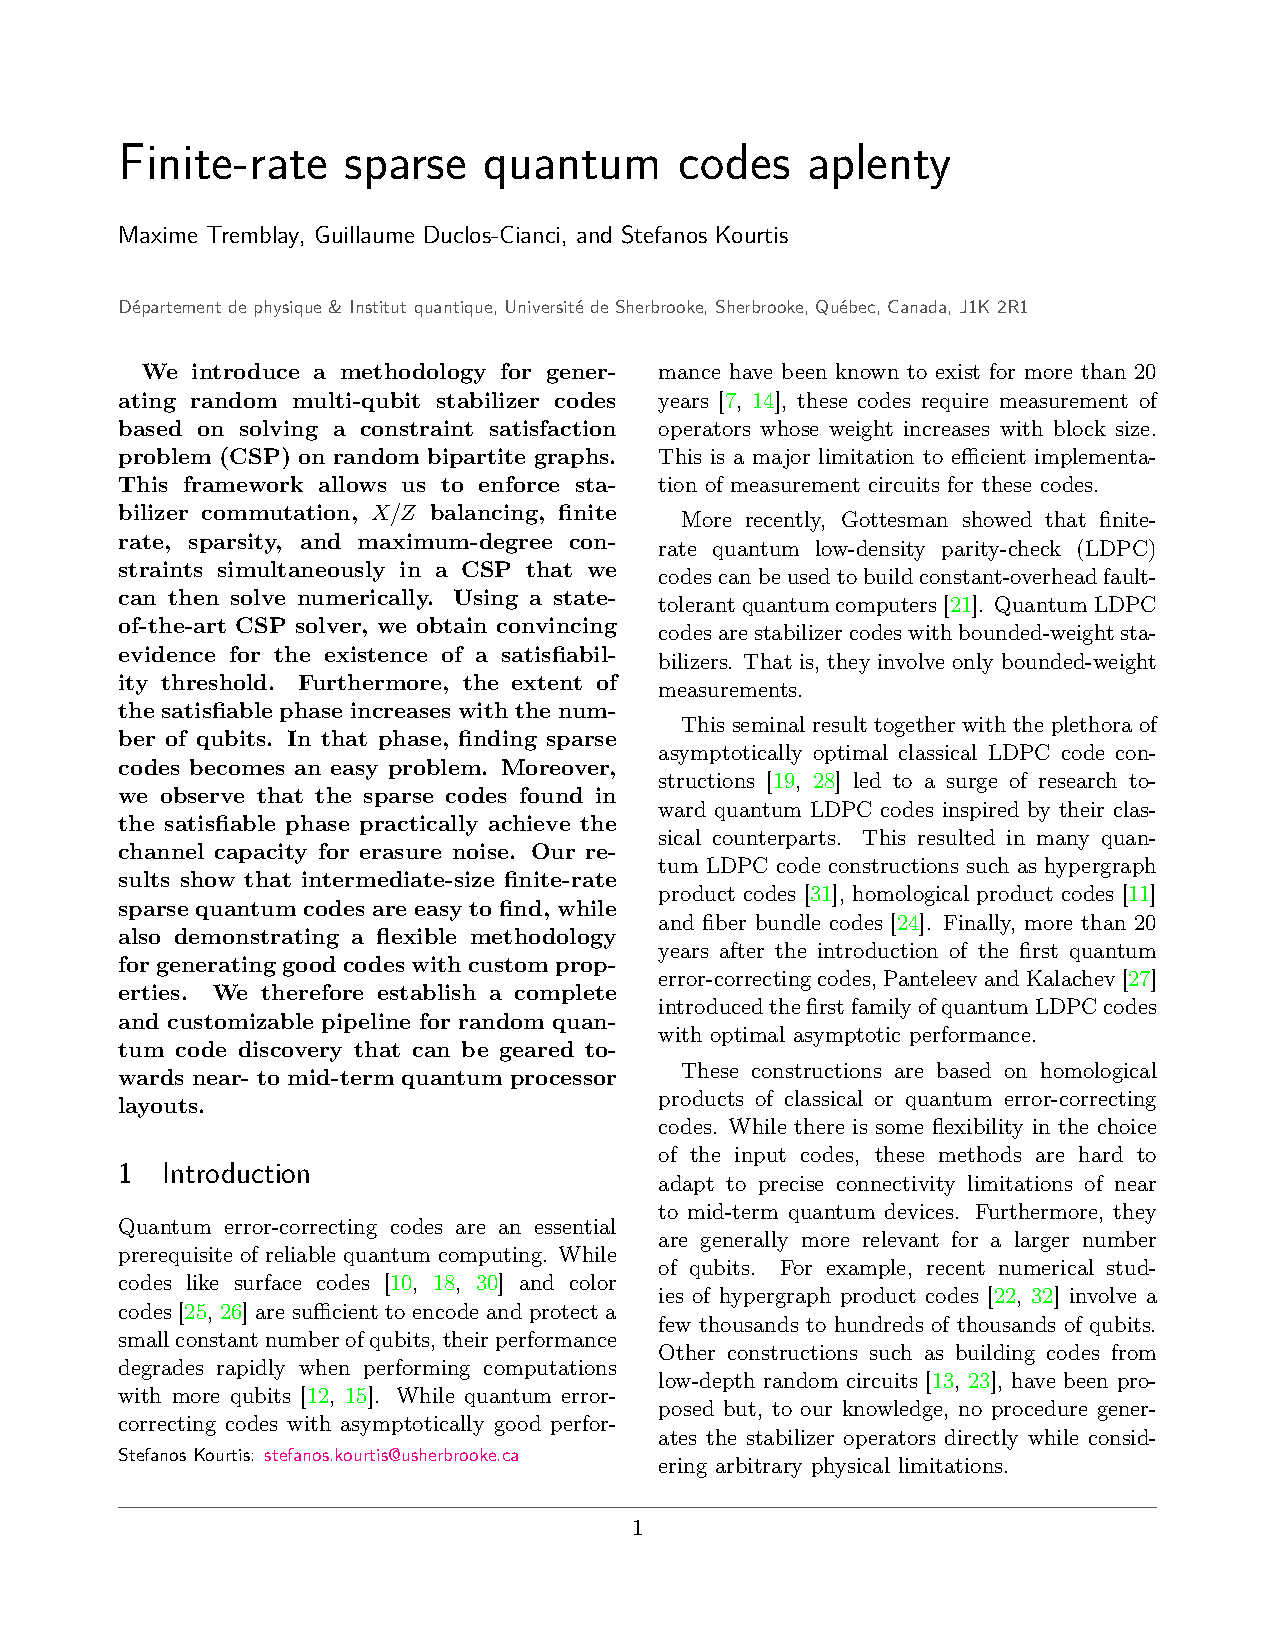
\includepdf[pages=-]{articles/sat_codes_construction.pdf}


\begin{comment}
\end{comment}

\chapter{Circuits pour la tolérance aux fautes quantique}

Pour terminer le récit de ma thèse,
j'ajoute un niveau de réaliste au modèle de correction d'erreurs quantique
du chapitre précédent pour présenter la conception d'une mémoire quantique.
Une mémoire quantique est un système quantique que l'on utilise pour stocker
de l'information pour une durée indéterminée.
Cependant,
tel que mentionnée au chapitre précédent,
les systèmes quantiques sont sujets aux erreurs,
même lorsque aucune opération n'est effectuée.
Ainsi,
pour construire une mémoire quantique,
il est nécessaire, encore une fois,
d'utiliser un code correcteur pour corriger les erreurs au fur et à mesure
qu'elles affectent le système.
Du moins,
il faut s'assurer que les erreurs restent assez faibles afin de pouvoir utiliser
l'information stockée dans le système pour un calcul futur.

En principe,
il est possible d'utiliser n'importe quel code correcteur pour construire
une mémoire quantique,
mais certains ont des propriétées plus favorables.
D'abord,
il est difficile de mettre à l'échelle un code correcteur dont le graphe
de Tanner est local, soit un graphe où la distance entre chaque paire de sommets 
connectés par une arête est borné indépendemment du nombre de sommets.
Plus précisément,
Bravyi, Poulin et Terhal~\cite{bravyi_tradeoffs_2010}
ont montré que pour un tel code $[n, k]$,
la distance minimale $d$ est limitée par
\begin{equation}
	d^2 \leq c \frac{n}{k},
\end{equation}
pour une constante $c$.
Ainsi,
si $k$ augmente proportionnellement avec $n$,
la distance minimum est bornée par une constante.
De plus,
pour avoir une distance minimale raisonnable,
il est nécessaire que le nombre de qubits encodés $k$ 
soit constant.

Ce résultat implique que pour un grand $n$,
soit peu de qubits sont encodés,
soit ceux-ci sont mal protogés des erreurs.
Il est donc difficile d'utiliser ces codes pour construire une mémoire 
quantique de grande taille.
Cependant,
lorsque la contrainte de localité du graphe de Tanner est abandonnée,
Gottesman~\cite{gottesman_fault-tolerant_2013} a montré qu'il est possible 
de construire une mémoire quantique protégeant efficacement les erreurs,
avec $\frac{k}{n}$ constant, en utilisant des codes LDPC.
Conséquemment,
il est possible d'utiliser des codes LDPC pour construire 
des mémoires quantiques de grandes échelles.

D'un point de vue expérimentale,
les codes LDPC ont l'avantages de pouvoir être implémenté de sorte que 
chaque qubit soit connecté à un nombre bornée d'autres qubits.
Comme je le présenterai plus tard lorsque j'introduirai les circuits
de mesures de syndromes,
cela permet d'implémenter efficacement les circuits nécessaires à la
construction d'une mémoire quantique,
à la condition de pouvoir coupler n'importe quelle paire de qubits 
indépendemment de la distance qui les sépares.











\section{Tolérance aux fautes quantique}

\section{Circuits extracteurs de syndromes}

\section{Codes de produits d'hypergraphes et codes expanseurs}

\section{Article}

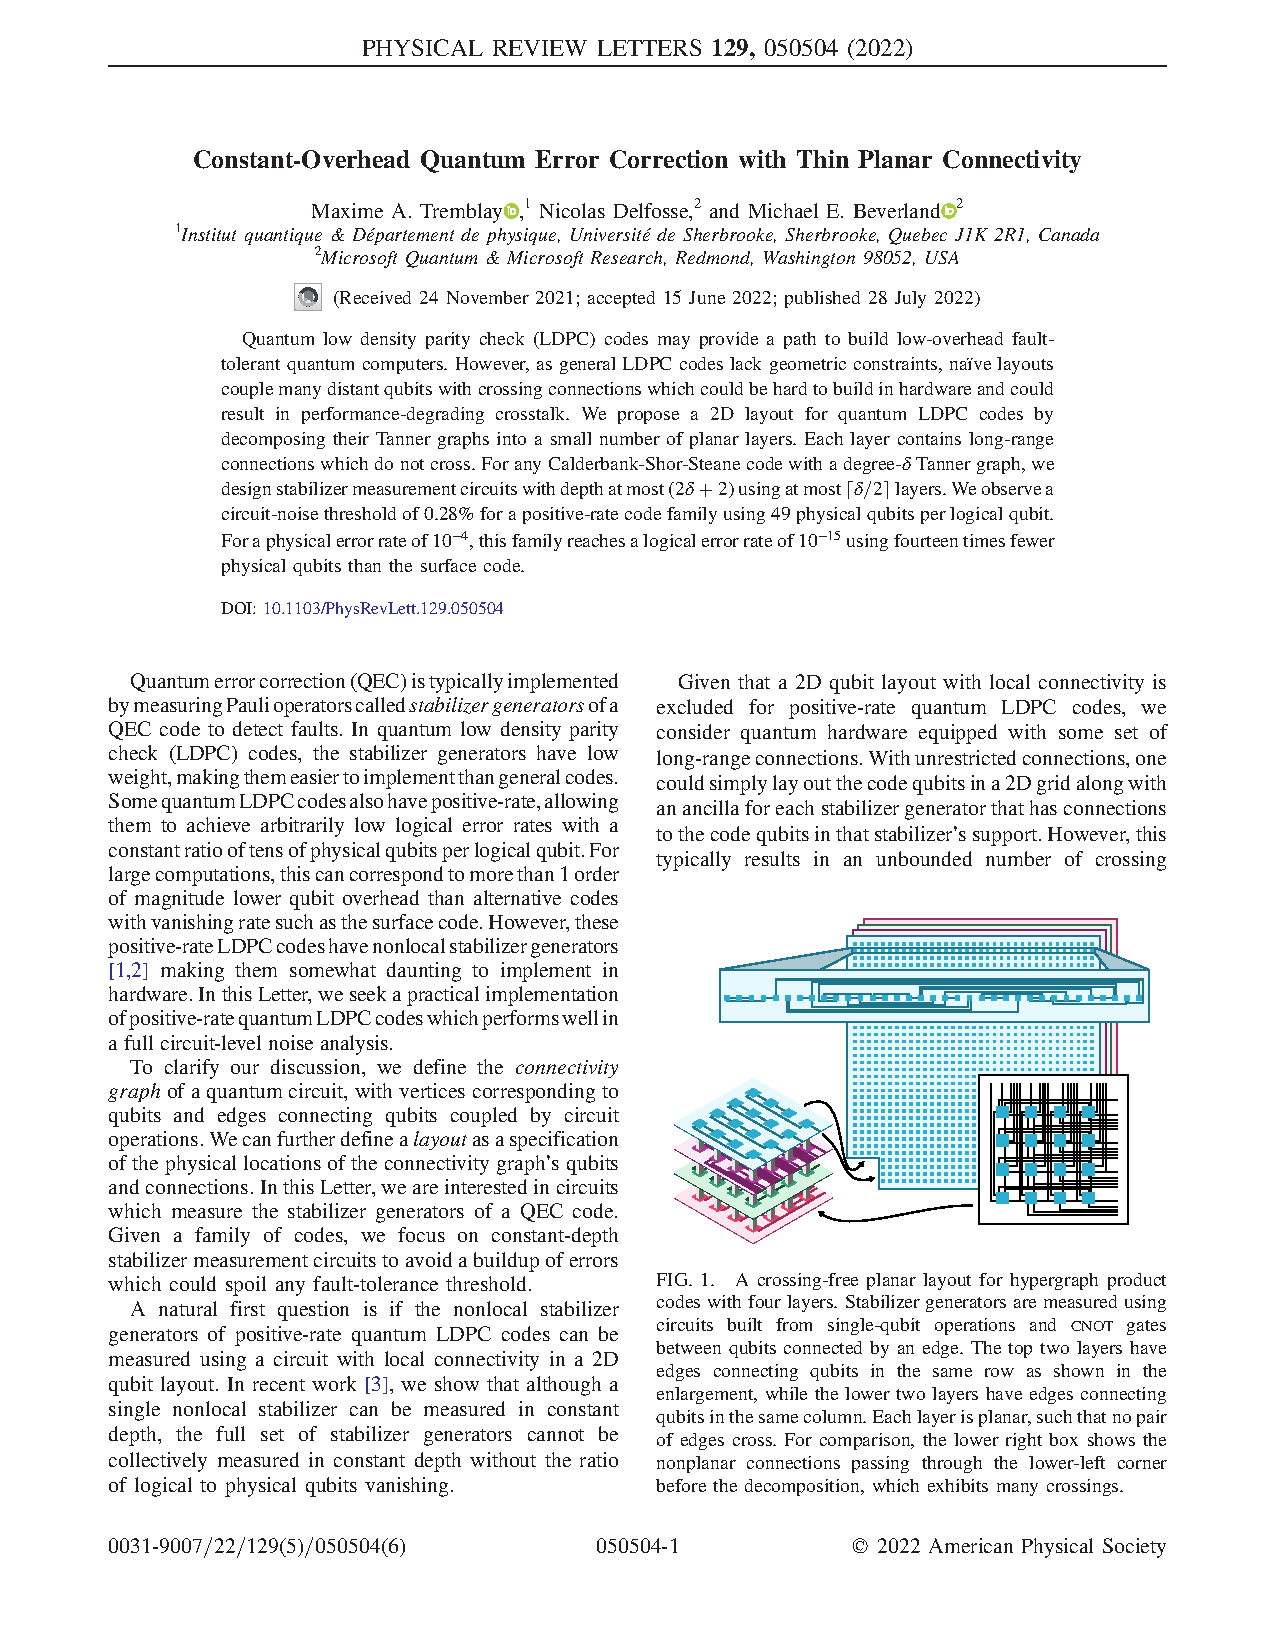
\includepdf[pages=-]{articles/planar_layout.pdf}



\begin{comment}
\end{comment}

\Conclusion % Chapitre qui ne sera pas numéroté si IntroConcluSansNombre est Vrai

Dans cette thèse,
j'ai présenté trois projets de recherche effectués lors de mon doctorat.
Tous ces projets traitent de la correction des erreurs,
mais dans des modèles de calcul différents.

Lors du premier projet,
j'ai mesuré l'impact de divers paramètres sur la performance et le temps de décodage
des codes polaires convolutifs.
Cela a permis d'identifier que les codes de profondeur et largeur deux offrent les
meilleures performances en fonction du temps de décodage.
Ce résultat pousse donc plus loin les performances des codes polaires standards
qui sont présentement utilisés dans le réseau de communication 5G.
Bien que les considérations d'ingénierie d'un réseau de communication sortent du cadre de cette thèse,
il est évident que toutes les améliorations à la correction d'erreurs peuvent réduire les 
couts d'implémentation d'un tel réseau.
En effet,
comme le taux d'erreur dépend de la distance entre les antennes,
un code qui permet de corriger plus d'erreurs permet également d'augmenter la distance
entre les antennes ce qui engendre une réduction du nombre nécessaire.

Le second projet que j'ai présenté est en réalité le dernier que j'ai effectué.
Dans le cadre de celui-ci,
je me suis intéressé à la construction de codes correcteurs quantiques.
La contribution la plus importante de ce projet réside dans la connexion
entre les problèmes de satisfaction de contraintes et la construction de codes.
Cela a permis de numériquement démontrer l'existence d'un seuil de satisfaisabilité
pour la probabilité d'inclusion d'une arête dans le graphe de support,
au-delà duquel il est facile de trouver des codes.
Il existe donc des régimes de paramètres pour lesquels il est aisé de construire des codes.
De plus,
j'ai poussé la méthode plus loin pour construire une famille de codes LDPC offrant des 
performances optimales pour le canal à effacement.
Il reste encore du chemin à faire,
mais cette approche offre la possibilité de découvrir des codes correcteurs pouvant être
adaptés aux contraintes physiques des ordinateurs quantiques à court et moyen terme.

Le troisième projet dont j'ai traité s'intéresse à la réalisation d'une architecture
permettant l'implémentation d'une mémoire quantique.
Des simulations numériques montrent également que cette approche permet de réduire significativement
le nombre de qubits nécessaires.
Bien sûr,
il reste de nombreux défis à résoudre pour implémenter cette architecture en laboratoire,
notamment l'implémentation de connexions à longue portée entre les qubits.
Tout de même,
l'approche présentée permet d'éliminer les croisements entre les connexions en exploitant
un petit nombre de couches dans la troisième dimension.
De plus,
les méthodes de traçage de graphes utilisées pour obtenir cette architecture 
ont le potentiel d'être appliquées pour contourner d'autres limitations à l'implémentation
du calcul tolérant aux fautes.

Dans l'ensemble de ces projets,
les modèles de bruits étudiés demeurent agnostiques de la technologie utilisée pour construire
les qubits.
Ce choix est fait puisqu'il est encore trop tôt pour choisir une technologie parmi toutes celles
proposées.
Il reste donc du travail à faire pour adapter les méthodes proposées dans cette thèse aux diverses 
technologies de qubits.
Cependant,
les travaux de cette thèse démontrent bien comment il est possible d'utiliser divers outils,
des réseaux de tenseurs aux méthodes de traçage de graphes en passant par les problèmes de satisfaction
de contraintes,
pour faciliter le design de systèmes quantiques tolérant aux fautes.


%-----------------------------------------------------------------------------%

% Voir switchboard.tex pour le bibliographystyle selon le type de document.
\bibliography{references}        % Le fichier de bibliographie est memoire.bib.

\singlespacing

\begin{comment}
\end{comment}

\appendix
% \renewcommand\chapterstring{Annexe}

\chapter{Théorie de l'information}
\label{chap:theo_info}

Considérant une variable aléatoire $X$ dont les valeurs possibles sont les éléments de $\mathcal X$
avec probabilité $\Pr: \mathcal X \to [0, 1]$,
la quantité d'information acquise après une réalisation $x \in \mathcal X$ de cette variable
est $\log(1/\Pr(x))$.
L'\textbf{entropie de Shannon} est l'espérance de cette valeur, soit 
\begin{align}
  H(X) = \mathbb E\qty(\log\qty(\frac{1}{\Pr(X)})) = -\sum_{x\in\mathcal X}\Pr(x) \log(\Pr (x)).
\end{align}
Dans cette définition,
il est considéré que $p\log(p) = 0$ lorsque $p = 0$.

Pour deux variables aléatoires $X, Y$ de domaines $\mathcal X, \mathcal Y$,
l'\textbf{entropie conjointe} est 
\begin{align}
  H(X, Y) 
  = \mathbb E\qty(\log\qty(\frac{1}{\Pr(X, Y)})) 
  = -\sum_{x\in\mathcal X, y \in\mathcal Y}\Pr(x, y) \log(\Pr(x, y))
\end{align}
et l'\textbf{entropie conditionnelle} est
\begin{align}
  H(X | Y) 
  = \mathbb E\qty(\log\qty(\frac{1}{\Pr(X|Y)})) 
  = -\sum_{x\in\mathcal X, y \in\mathcal Y}\Pr(x, y) \log(\Pr(x|y)).
\end{align}
Il est aisé de vérifier que 
\begin{align}
  H(X, Y) = H(X | Y) + H(Y) = H(Y | X) + H(X).
\end{align}
Ainsi,
l'information acquise après la réalisation simultanée de deux variables aléatoires
est équivalente à la somme de l'information acquise en réalisant la première 
et de l'information acquise en réalisant la seconde en connaissant la valeur de la première.

L'\textbf{information mutuelle} entre deux variables aléatoires $X, Y$ est
l'information que révèle une réalisation d'une des variables sur l'autre variable.
L'information mutuelle se mesure en comparant la probabilité conjointe de $X, Y$
aux probabilités marginales, soit
\begin{align}
  I(X ; Y) 
  &= \mathbb E\qty(
    \log\qty(\frac{1}{\Pr(X)\Pr(Y)})
    -
    \log\qty(\frac{1}{\Pr(X, Y)})
  ) \notag \\
  &= -\sum_{x\in\mathcal X, y \in\mathcal Y}\Pr(x, y) \log(\frac{\Pr(X, Y)}{\Pr(X)\Pr(Y)}).
\end{align}
Cette définition est symétrique,
c'est-à-dire $I(X ; Y) = I(Y ; X)$.
De plus,
l'information mutuelle est reliée aux diverses entropies selon
\begin{align}
  I(X;Y)
  = H(X) - H(X | Y)
  = H(Y) - H(Y | X)
  = H(X) + H(Y) - H(X, Y).
\end{align}
Le première équation illustre bien que l'information mutuelle correspond à la différence
d'information acquise par une réalisation de $X$ lorsque $Y$ est inconnue ou connue.


\chapter{Théorie des graphes}
\label{chap:theo_graphe}

Un \textbf{graphe} est une paire $(S, A)$ telle que 
\begin{align}
  A \subseteq \qty{\qty{s, t} : s,t \in S}.
\end{align}
Les éléments de $S$ se nomment \textbf{sommets}
et les éléments de $A$ se nomment \textbf{arêtes}.
Deux sommets $s, t \in S$ sont \textbf{connectés} si $\qty{s, t} \in A$.
Le \textbf{voisinage} d'un sommet $s$ est l'ensemble des arêtes contenant $s$,
soit 
\begin{align}
  \eta(s) = \qty{a \in A : s \in a}.
\end{align}
Le \textbf{degré} d'un sommet est la taille de son voisinage.

Un \textbf{graphe biparti} est un graphe pour lequel il existe une 
partition des sommets $S = U \cup V$ telle que 
\begin{align}
  A \subseteq \qty{\qty{u, v} : u \in U,\, v \in V}.
\end{align}
Ainsi, les arêtes sont restreintes entre les paires de sommets n'appartenant pas
au même ensemble.
Un \textbf{hypergraphe} est une généralisation d'un graphe
où le nombre de sommets par arête est arbitraire.
Ainsi,
un hypergraphe est une paire $(S, A)$ telle que
\begin{align}
  A \subseteq \qty{X \subseteq S}.
\end{align}
Le voisinage et le degré d'un sommet sont définis de façon similaire à un graphe.
De plus, le poids $|a|$ de $a \in A$ est le nombre de sommets de cette arête.

Il existe une correspondance entre les graphes bipartis et les hypergraphes.
Pour un hypergraphe $H = (S, A)$,
la fonction 
\begin{align}
  \phi(H) = (S \cup A, B),
\end{align}
avec $\qty{s, a} \in B$ si $s \in a$,
est bijective et associe à chaque hypergraphe un unique graphe biparti.

Un \textbf{cycle} de longueur $n$ est un graphe $C_n = (S, A)$
avec $S = \qty{s_1, s_2, \ldots, s_n}$ et 
$A = \qty{\qty{s_1, s_2}, \qty{s_2, s_3}, \ldots, \qty{s_n, s_1}}$.
Un cycle de longueur paire est un graphe biparti.

Soit deux graphes $G = (S, A)$ et $H = (T, B)$,
le \textbf{produit cartésien} $G \times H$ est un graphe $(S \times T, C)$
tel que $\qty{(s_1, t_1), (s_2, t_2)} \in C$ si 
$s_1 = s_2$ et $\qty{t_1, t_2} \in B$ ou si $t_1 = t_2$ et $\qty{s_1, s_2} \in A$.
Le produit cartésien de deux graphes contenant chacun deux sommets et une arête reliant ces
sommets est un cycle de longueur quatre.
Ainsi,
pour le produit cartésien $G \times H$,
chaque paire d'arêtes $a \in A$ et $b \in B$ engendre un cycle de longueur quatre dans $C$.

\chapter{Complexité de calcul}
\label{chap:complexite_calcul}

Dans cette section,
la rigueur des définitions est variable.
Définir formellement la complexité de calcul demande d'introduire un modèle de 
calcul comme la machine de Turing.
Cependant,
cela sort beaucoup du cadre de cette thèse
et je me contente de définitions qui sont suffisantes à la compréhension du contenu de la thèse
et j'évite plusieurs détails.

Un \textbf{problème de calcul} est représenté par une relation $R \subseteq X \times Y$, 
où $X$ est l'ensemble des \textbf{entrées} et $Y$ est l'ensemble des \textbf{solutions}.
Les solutions de $x \in X$ sont les éléments de l'ensemble $Y_R(x) = \qty{y \in Y : (x, y)\in R}$.
Un \textbf{algorithme} $a: X \to Y$ résout $R$ si $a(x) \in Y_R(x)$ pour tous $x \in X$.

Un algorithme se décompose en une série d'opérations $a_1, \ldots a_c \in \mathcal A$ telle
que $a(x) = (a_c \circ \ldots \circ a_1)(x)$ où $\circ$ représente la composition
de fonctions.
Cette décomposition de $a$ varie en fonction de la taille de $x$
et dépend également des opérations accessibles $\mathcal A$.
Plus précisément,
il est supposé que les entrées $X$ sont décrites par des listes de tailles variées
d'éléments d'un alphabet $\mathcal X$.
Ainsi,
$X \subseteq \mathcal X^* = \cup_{n=0}^\infty \mathcal X^n$ et
une entrée $x \in X$ a une taille $n$ si $x \in \mathcal X^n$.

La \textbf{complexité} d'un algorithme est le nombre $c(n)$ d'opérations nécessaires
pour calculer $a(x)$ selon la taille $n$ de $x$.
Il est souvent difficile et peu pertinent de calculer la valeur exacte de $c(n)$
et il est généralement suffisant de connaitre le comportement général de $c(n)$.
Pour ce faire,
nous utilisons la \textbf{notation grand $\mathcal O$}.
Une fonction $f(n)$ a la complexité $\mathcal O(g(n))$ s'il existe
une constante $k$ telle que $f(n) \leq k g(n)$.
Généralement,
les complexités considérées sont les complexités \textbf{logarithmiques} $\mathcal O(\log n)$,
\textbf{linéaire} $\mathcal O(n)$,
\textbf{polynomiale} $\mathcal O(n^t)$ pour un entier $t > 0$
et \textbf{exponentielle} $\mathcal O(2^n)$.

Par exemple,
le problème du tri d'une liste d'entiers est défini par la relation
$R \subseteq \mathbb Z^* \times \mathbb Z^*$
où chaque paire $(x, y) \in R$ est une liste $x$ et sa version triée $y$.
Les opérations disponibles pour trier une liste sont la permutation et
la comparaison de deux éléments.
Comme il y a $n(n-1)/2$ paires de nombre,
un algorithme naif de tri a une complexité $\mathcal O(n^2)$.

Dans cette thèse,
j'utilise trois classes de complexité importantes.
Premièrement,
la \textbf{classe P} est l'ensemble des problèmes
pour lesquels il existe un algorithme de complexité polynomiale.
Deuxièmement,
la \textbf{classe NP} est l'ensemble des problèmes
pour lesquels il existe un algorithme de complexité polynomiale
qui permet de vérifier qu'une paire $(x, y)$ satisfait la relation.
La différence avec la classe P est qu'il n'est pas nécessaire qu'un 
algorithme de complexité polynomial soit en mesure de trouver $y \in Y_R(x)$,
mais seulement qu'un algorithme soit en mesure de vérifier que $y$ est une solution
de $x$.
Troisièmement,
un problème de la \textbf{classe $\sharp$P} est défini à partir d'un problème
$R = (X, Y)$ de la classe NP.
Le problème $N = (X, Y_R(X))$ de $\sharp$P correspondant est le problème de
recherche du nombre de solutions dans $R$ d'une entrée $x \in X$.

Évidemment, $\text{P} \subseteq \text{NP}$.
Par contre, 
il est toujours une question ouverte de déterminer si
$\text{P} \subset \text{NP}$ ou si $\text{P} = \text{NP}$.
Par contre,
la conjecture la plus acceptée est que $\text{P} \subset \text{NP}$.

Un problème $R = (X_R, Y)$ est \textbf{complet} pour une classe de complexité
si pour tout problème $S = (X_S, Y)$ de cette classe il existe une fonction 
$f: X_S \to X_R$ de complexité polynomiale.
En particulier,
un problème $R$ est \textbf{NP-complet} si un algorithme $A$ pour $R$
permet de construire, avec un surcout polynomial,
un algorithme pour résoudre un problème arbitraire de NP.

\chapter{Théorie des groupes}
\label{chap:theo_groupes}

Un \textbf{groupe} $(G, *)$ est un ensemble $G$ avec une opération $* : G \times G \to G$
satisfaisant les trois conditions suivantes.
L'opération $*$ est associative.
Il existe un élément identité $e$ tel que $e * g = g * e = g$ pour tous $g \in G$.
Chaque élement $g \in G$ a un inverse $g^{-1} \in G$ tel que $g * g^{-1} = g^{-1} * g = e$.
Par exemple $(\mathbb Z, +)$ est le groupe des nombres entiers avec l'opérateur d'addition.
De plus, un groupe est \textbf{abélien} si l'opération est commutative.

Les groupes considérés dans la thèse sont tous des groupes multiplicatifs.
Dans ce cas, l'opérateur est noté $\cdot$ et régulièrement omis.
Ainsi, $gh$ et $g \cdot h$ sont deux notations équivalentes pour la multiplication 
de deux éléments d'un groupe.
Comme l'opération est sous-entendu,
il est commun de noter un groupe $(G, \cdot)$ seulement à partir de l'ensemble $G$.

La \textbf{cardinalité} $|G|$ d'un groupe $G$ est le nombre d'éléments de celui-ci.
Les groupes considérés dans la thèse ont tous une cardinalité finie.
Un \textbf{sous-groupe} est un sous-ensemble $H \subseteq G$ satisfaisant les trois conditions
d'un groupe.
Je note alors $H \sqsubseteq G$.
Un sous-ensemble $S \subseteq G$ est un \textbf{générateur} d'un sous-groupe $H$ si $H$ est le plus petit
sous-groupe contenant $S$.
J'utilise $g(H)$ pour représenter un générateur de $H$ 
et $\langle S \rangle$ pour représenter le sous-groupe généré par $S$.
Les éléments d'un sous-ensemble $S \subseteq G$ sont \textbf{indépendants} si 
$|\langle T \rangle| < |\langle S \rangle|$ pour tous $T \subset S$.

Pour $H \sqsubseteq G$,
la \textbf{classe à gauche} d'un élément $g \in G$ est
\begin{align}
  gH = \qty{gh : h \in H}.
\end{align}
De même,
la \textbf{classe à droite} de $g$ est 
\begin{align}
  Hg = \qty{hg : h \in H}.
\end{align}
Si $Hg = gH$ pour tous $g \in G$,
alors $H$ est un \textbf{sous-groupe normal} et,
pour tous $f, g \in G$, l'opération
\begin{align}
  (fH)\cdot(gH) = (fg)H
\end{align}
entre les classes de $H$ respecte la définition d'un groupe.
Cela permet de former le \textbf{groupe quotient} 
\begin{align}
  G / H = \qty{gH : g \in G},
\end{align}
soit le groupe des classes de $H$.

La \textbf{conjugaison} de $g \in G$ et $H \sqsubseteq G$ est 
\begin{align}
  gHg^{-1} = \qty{ghg^{-1} : h \in H}.
\end{align}
Le \textbf{normalisateur} de $H$ est l'ensemble des éléments de $G$ qui laisse $H$
invariant après conjugaison.
C'est-à-dire, l'ensemble
\begin{align}
  \mathcal{N}_G(H) = \qty{g \in G : gHg^{-1} = H}.
\end{align}
Le \textbf{centralisateur} de $H$ est l'ensemble des éléments de $G$ qui commutent avec
tous les éléments de $H$, soit
\begin{align}
  \mathcal{C}_G(H) = \qty{g \in G : gh = hg,\, h \in H}.
\end{align}
Il est toujours vrai que $\mathcal{C}_G(H) \subseteq \mathcal{N}_G(H)$ puisque
si $g \in \mathcal{C}_G(H)$ alors $ghg^{-1} = hgg^{-1} = h$.

Soit un groupe $G$ tel que $fg = \pm gf$ pour tous $f,g \in G$
et $H \sqsubseteq G$ tel que $h \in H \implies -h \not\in H$,
alors $\mathcal{N}_G(H) = \mathcal{C}_G(H)$ puisque
\begin{align}
  ghg^{-1} = \pm hgg^{-1} = \pm h = h
\end{align}
pour tous $h \in H$.
Ceci est le cas pour le groupe stabilisateur présenté au chapitre~\ref{chap:construction_codes}
de cette thèse.


%=============================================================================%


\end{document}
